% Options for packages loaded elsewhere
\PassOptionsToPackage{unicode}{hyperref}
\PassOptionsToPackage{hyphens}{url}
%
\documentclass[
]{book}
\usepackage{amsmath,amssymb}
\usepackage{lmodern}
\usepackage{iftex}
\ifPDFTeX
  \usepackage[T1]{fontenc}
  \usepackage[utf8]{inputenc}
  \usepackage{textcomp} % provide euro and other symbols
\else % if luatex or xetex
  \usepackage{unicode-math}
  \defaultfontfeatures{Scale=MatchLowercase}
  \defaultfontfeatures[\rmfamily]{Ligatures=TeX,Scale=1}
\fi
% Use upquote if available, for straight quotes in verbatim environments
\IfFileExists{upquote.sty}{\usepackage{upquote}}{}
\IfFileExists{microtype.sty}{% use microtype if available
  \usepackage[]{microtype}
  \UseMicrotypeSet[protrusion]{basicmath} % disable protrusion for tt fonts
}{}
\makeatletter
\@ifundefined{KOMAClassName}{% if non-KOMA class
  \IfFileExists{parskip.sty}{%
    \usepackage{parskip}
  }{% else
    \setlength{\parindent}{0pt}
    \setlength{\parskip}{6pt plus 2pt minus 1pt}}
}{% if KOMA class
  \KOMAoptions{parskip=half}}
\makeatother
\usepackage{xcolor}
\usepackage{longtable,booktabs,array}
\usepackage{calc} % for calculating minipage widths
% Correct order of tables after \paragraph or \subparagraph
\usepackage{etoolbox}
\makeatletter
\patchcmd\longtable{\par}{\if@noskipsec\mbox{}\fi\par}{}{}
\makeatother
% Allow footnotes in longtable head/foot
\IfFileExists{footnotehyper.sty}{\usepackage{footnotehyper}}{\usepackage{footnote}}
\makesavenoteenv{longtable}
\usepackage{graphicx}
\makeatletter
\def\maxwidth{\ifdim\Gin@nat@width>\linewidth\linewidth\else\Gin@nat@width\fi}
\def\maxheight{\ifdim\Gin@nat@height>\textheight\textheight\else\Gin@nat@height\fi}
\makeatother
% Scale images if necessary, so that they will not overflow the page
% margins by default, and it is still possible to overwrite the defaults
% using explicit options in \includegraphics[width, height, ...]{}
\setkeys{Gin}{width=\maxwidth,height=\maxheight,keepaspectratio}
% Set default figure placement to htbp
\makeatletter
\def\fps@figure{htbp}
\makeatother
\setlength{\emergencystretch}{3em} % prevent overfull lines
\providecommand{\tightlist}{%
  \setlength{\itemsep}{0pt}\setlength{\parskip}{0pt}}
\setcounter{secnumdepth}{5}
\usepackage{booktabs}
\ifLuaTeX
  \usepackage{selnolig}  % disable illegal ligatures
\fi
\usepackage[]{natbib}
\bibliographystyle{apalike}
\IfFileExists{bookmark.sty}{\usepackage{bookmark}}{\usepackage{hyperref}}
\IfFileExists{xurl.sty}{\usepackage{xurl}}{} % add URL line breaks if available
\urlstyle{same} % disable monospaced font for URLs
\hypersetup{
  pdftitle={Hizkuntzaren Didaktika (2022) Haur Hezkuntza V0.2},
  pdfauthor={Juan Abasolo},
  hidelinks,
  pdfcreator={LaTeX via pandoc}}

\title{Hizkuntzaren Didaktika (2022) Haur Hezkuntza V0.2}
\author{Juan Abasolo}
\date{2022-10-20}

\begin{document}
\maketitle

{
\setcounter{tocdepth}{1}
\tableofcontents
}
\hypertarget{Aurretikoak}{%
\chapter*{Aurretikoak}\label{Aurretikoak}}
\addcontentsline{toc}{chapter}{Aurretikoak}

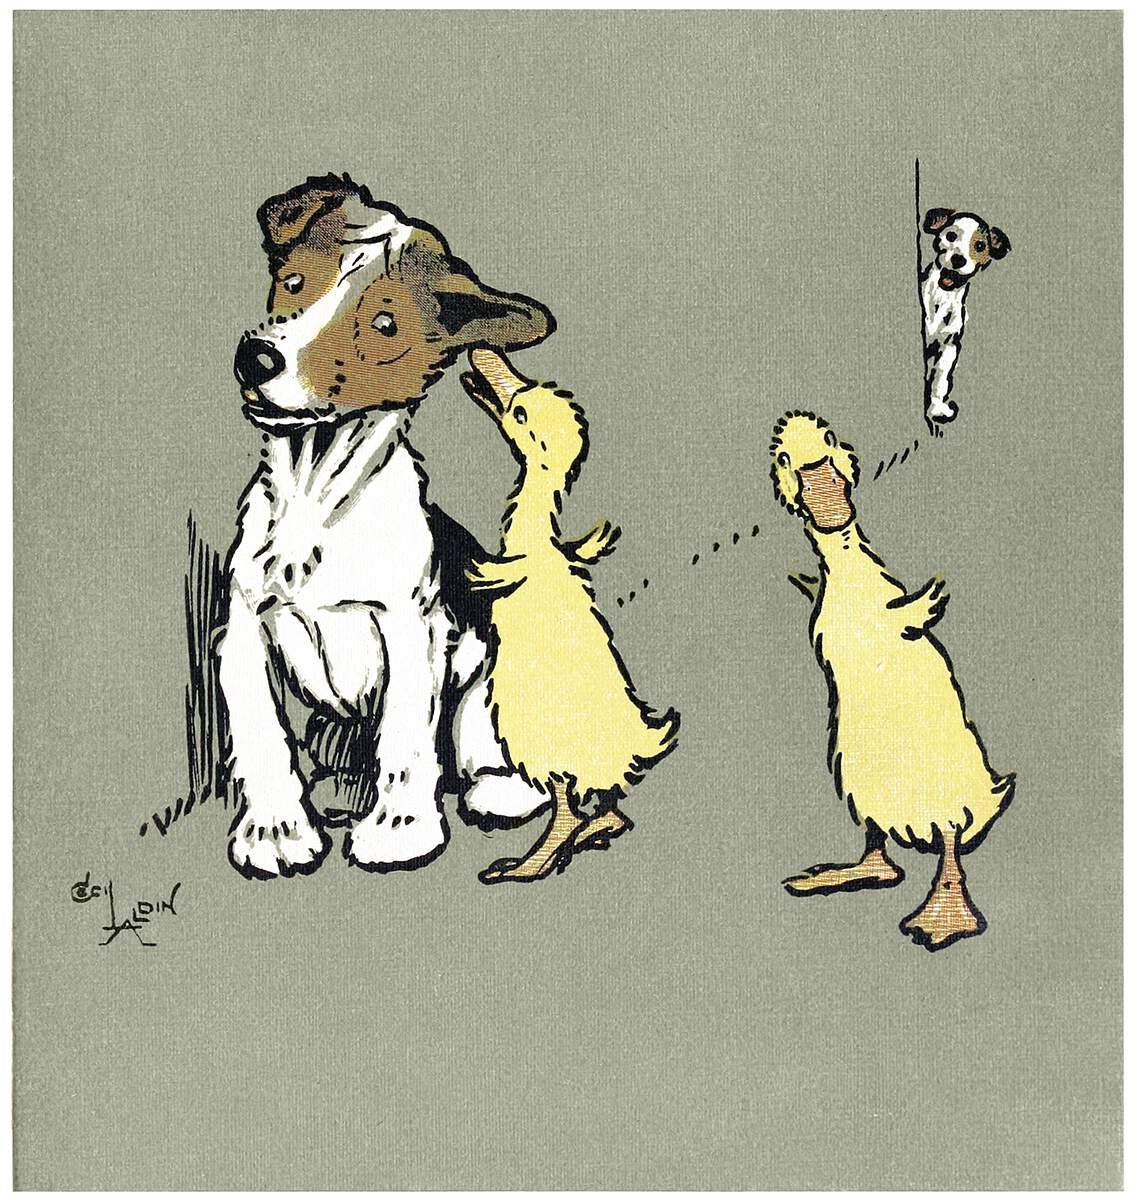
\includegraphics{assets/scare-quacks-1200.jpg}

Hizkuntzaren Didaktika eta Atzerriko Hizkuntza ikasgaiko lehenengo zatiko apunteak daude hemen, Hizkuntzaren Didaktikako zatikoak, hain zuzen.

Hamar astean zehar antolatzen dira ikasgai honetako eskolak, honela 2020 urtean, ahaleginez:

\begin{enumerate}
\def\labelenumi{\arabic{enumi}.}
\tightlist
\item
  astea: Aurkezpen eguna \href{../diapoak/}{*}
\item
  astea: Zer da Hizkuntza \textbar{} Hizkuntzalaritza
\item
  astea: Hizkuntzalaritza
\item
  astea: Nola ikasten du umeak hizketan \textbar{} Proiektuaren aurkezpena
\item
  astea: Hizkuntza patologiak
\item
  astea: Hizkuntza patologiak \textbar{} Ahozko hizkuntza haur hezkuntzan
\item
  astea: Ahozko hizkuntza haur hezkuntzan
\item
  astea: Ahozko hizkuntza haur hezkuntzan
\item
  astea: Murgiltze klaseak
\item
  astea: Aurkezpenak eta azterketarako azken prestaketak
\end{enumerate}

Hobeto eta sakonago irakur dezakezu \href{../Baliabideak/00_aurkezpena/Syllabus_HDHH22-V0.pdf}{hemen}.

\begin{center}\rule{0.5\linewidth}{0.5pt}\end{center}

Jakin beza hona iritsitako nabigatzaileak apunteok ez direla egile honek egindakoak, baizik eta hainbaten lanetatik aurtengo ikasleentzat sortutako gunea.
Batez ere Asier Romerok, Karlak eta Lorea Unamunoren lanetatik edan dute apunteok.

\hypertarget{T1}{%
\chapter{Zer da hizkuntza?}\label{T1}}

Hizkuntza zer den definitu behar genuke, hizkuntzaren didaktikaz aritu behar dugula esan aurretik. Baina hizkuntza zer den argi, garbi eta ezbairik gabe esaten duenik ere ez dakigu dagoen.

Hizkuntza hitz egiten dugunean, zer datorkigu burura?

\begin{itemize}
\tightlist
\item
  Zer da hizkuntza bat?
\item
  Hizkuntza ikasten dugu? Ala beste zerbait gertatzen da? Zer?
\item
  Ama Hizkuntza edo etxeko hizkuntza eta beste guztiak berdin lortzen ditugu? Berdin lortzen dugu jakitea, alegia?
\item
  Eta berdin umetan edo nagusitan?
\item
  Etxean ikasten badugu hizkuntza, eskolan zer egiten dugu? Zein alde dago batetik bestera?
\end{itemize}

Esan dezakegu hizkuntza dela komunikazio tresna, pentsatzeko tresna, ikasteko tresna, sortzeko tresna\ldots{}

Erabaki behar dugu ea tresna den hizkuntza ala gu garen hizkuntzarenak. Zein neurritan den hori, behintzat.

\hypertarget{hizkuntza-komunikazio-tresna}{%
\section{Hizkuntza: komunikazio tresna}\label{hizkuntza-komunikazio-tresna}}

Gizakion arteko hartu-emanak erregulatzeko eta kontrolatzeko hizkuntza darabilgu.

Tresna posibleen artean eraginkorrena dela esan dezakegu, oso esanahi konplexuak adieraz ditzakegu baliabide urriko gastua eginaz. Gizakiok hizkuntzaren erabileraz ``orain'' eta ``hemen'' egotea gaindi dezakegu animaliek ezin dezaketen moduan.

\begin{quote}
Komunikatzea soilik ez, zer komunikatzen den ere kontuan izan bhear da. Partikulazki, lengoaiaren bitartez baino ezin daitekeena komunikatu

-- Tough, \emph{El lenguage oral en la escuela}, 14. orr. (JAk itzulia)
\end{quote}

\hypertarget{hizkuntza-pentsatzeko-eta-ikasteko-tresna}{%
\section{Hizkuntza: pentsatzeko eta ikasteko tresna}\label{hizkuntza-pentsatzeko-eta-ikasteko-tresna}}

Hizkuntzaren bitartez mundua ezagutzen eta ulertzen dugu, hizkuntzak berak horretan laguntzen digulako.

Munduan eragiteko hizkuntza darabilgu jarduerak hizkuntzaren bitartez planifikatzen, antolatzen eta kontrolatzen ditugunean.

\begin{quote}
\ldots{} lengoaiaren bitartez, amak umeari erakusten dizkio eraiki behar duen munduaren planu semantikoak. Errealitate gordina ez daiteke habitatu: zentzua eman behar zaio, zatitu, alor eta sailetan banatu behar da eta euren arteko bideak eta hartu-emanak eraiki behar dira, batetik bestera igarotzeko. Nahitanahiez, haurrak eraiki behar du bere bizi-gunea, errealitatearen jabe egin behar baita. Baina latza litzateke arkitektura bera ere asmatu beharra. (\ldots) Hizkuntzari eskerrak, zure esperientzien menpekoa ez zara soilik, beste guztien eserientziak ere baliatu ditzakezu.

Hizkuntzak, norbanakoari Mundua eraikitzen uzteaz gain, horren jabe egiten ere uzten du. \ldots{} Amak ez dio soilik ordena ezartzen mundu objektiboari, haurraren subjekturik gabeko subjetibotasunari ere ezartzen dio \ldots{} Lengoaia, besteekiko komunikatzeko bitarteko legez hasten dena, umea bere buruarekin komunikatzeko bitarteko bilakatzen da, egintzak antolatzen lagunduaz. Adimena eraikitzeko berebiziko garrantzia du hizkuntzaren funtzio antolatzaileak.

-- Marina (1993), El mundo y el lenguaje, \emph{Teoría de la inteligencia creadora} (JAk itzulia)
\end{quote}

\begin{quote}
\ldots{} A través del lenguaje, la madre le enseña al niño los planes semánticos del mundo que tiene que construir. La cruda realidad no es habitable: hay que darle sentido, segmentarla, dividirla en estancias y construir pasillos y relaciones para pasar de uno a otro. Es la niña la que tiene que construir su hogar de manera irremediable, ya que necesita apropiarse de la realidad, pero sería un gran fastidio si tuviera que inventar la arquitectura. (\ldots) gracias al idioma no dependerá solo de tu experiencia, sino que podrás aprovechar la experiencia de los demás.

\ldots{} El lenguaje, además de permitir que el sujeto construya el Mundo, le permite tomar posesión de sí mismo \ldots{} La madre no solo introduce orden en el mundo objetivo, sino también en la subjetividad sin sujeto del niño \ldots{} El lenguaje, que comienza como un medio de comunicación con los demás, se convierte en un medio para que el niño se comunique consigo mismo, ayudándole a regular sus acciones. Esta función reguladora es de enorme importancia para la construcción de inteligencia \ldots{}

-- Marina (1993), El mundo y el lenguaje, \emph{Teoría de la inteligencia creadora}
\end{quote}

Ideion adibide argigarri batzuk, ingelesetik ekarrita, Wells (1988) liburuan:

\begin{quote}
Elizabeth, lau urteko haurra, amari so dago, beheko suko errautsak pala batekin batu eta balde batera zelan botatzen dituen ikusten.

E: Zertarako egiten duzu hori?\\
M: Batzen eta kanpora eramaten babil, gero aitak ortuan zabaltzeko\\
E: Eta zertarako botako ditu ortuan?\\
M: Lurra ontzeko.\\
E: Eta horrela ondo hasiko dira landarak?\\
M: Bai.\\
E: Eta hori, zergatik?\\
M: Gogoan duzu aurrekoan azaldu nizula zuk denetarik jan behar duzula, arraultzak eta azak eta porru-patatak neska handia hazteko?\\
E: Bai.\\
M: Ba, landareek ere denetarik behar dute. Eta haiei ondo doakienetariko bat errautsa da.

-- Wells, \emph{Aprender a leer y escribir}, 79 or. (JAk itzulia)
\end{quote}

\begin{quote}
Elisabeth, a la edad de 4 años, observa a su madre, que recoge con una pala las cenizas del hogar y las hecha en un cubo:

E: ¿Para qué haces eso? M: La estoy recogiendo y llevándola afuera para que papá la eche por el jardín\\
E: ¿Por qué ha de echarlas por el jardín? M: Para que esté bien abonado.\\
E: ¿Así crecerá la hierba?\\
M: Sí.\\
E: Y eso ¿por qué?\\
M: ¿Te acuerdas que te expliqué que tú necesitas comer cosas distintas como huevos y col y budín de arroz para hacerte grande?\\
E: Sí.\\
M: Pues las plantas también necesitan cosas distintas. Y una de las cosas que les van bien es la ceniza.

-- Wells, \emph{Aprender a leer y escribir}, 79 or.
\end{quote}

\begin{center}\rule{0.5\linewidth}{0.5pt}\end{center}

\begin{quote}
James, hiru urte eta erdi duela, etxeko lorategian jolasean izan da. Amak etxera eraman nahi du galtzerdi eta zapata lokastuak aldatzera, baina, etxera sartzeko dagoela, txoria ikusten du:

M: Ea. Horrela, zapata bat jantzita.\\
J: Txoria ikusten dut.\\
M: Zer ikusi, bihotza??\\
J: Txoritxoa ikusten dut.\\
M (ahopeka): Hor? Kanpoan?\\
J (atzamarraz erakutsiaz eta ahopela):Bai. Ikusten dut\\
{[}Biek ahopeka segitzen dute{]}\\
M: Ezer jaten dabil?\\
E: Ez.\\
M: Han doa\ldots{} -txoritxoa paperezko bortsa batera doa eta zati batzuk hartzen ahalegintzen da- Oh, hor jateko apur bat dauka. Eta uste dut zatitxu batzuk hartuko dituela kabia egiteko. James, egon apur batean banoa\ldots{}

Jamesek hurbilagotik ikustera irten nahi du, baina momentu horretantxe txoritxoa hegaz hasten da.

J: Txoritxoa joan egin da.\\
M (tonu normalean): Joan egin da?\\
J: Bai.

-- Wells, \emph{Aprender a leer y escribir}, 81 or.
\end{quote}

\begin{quote}
James, a la edad de 3 años y medio, ha estado jugando en el jardín. Su madre quiere llevárselo para cambiarle los calcetines y los zapatos embarrados pero, al entrar, el niño ve un pájaro:

M: Vamos a ver. Así -- una zapatilla puesta.\\
J: Veo un pájaro.\\
M: ¿Un qué, cielo?\\
J: Veo un pájaro.\\
M (en un susurro): ¿Ahí? ¿Afuera?\\
J (señalando y susurrando): Sí. Lo veo. (Los dos siguen hablando en susurros)\\
M: ¿Se está comiendo algo?\\
E: No.\\
M: Va a la --la bolsa de papel a intentar coger unos trozos --Oh, ahí tiene un poco de comida. Y supongo que cogerá unos trozos de la bolsa para hacer su nido debajo del tejado. James, espera un poco que voy\ldots{}

James quiere salir a verlo más de cerca, pero en ese momento el pájaro alza el vuelo

J: El pájaro se ha ido.\\
M (hablando de nuevo a un volumen normal): ¿Ya se ha ido?\\
J: Sí.

-- Wells, \emph{Aprender a leer y escribir}, 81 or.
\end{quote}

\begin{quote}
Simonek, lau urte eta bederatzi hilekoa, sagarra jan berri du eta haziekien batu ditu. Amari azaltzen dio zer egin litekeen horiekin.

S: Hazia haz daiteke. Batzuk erein ahal ditugu. Sagar-hazi askotxu ditut eta, gehiago lortzen baditut, aitak eta biok egunen batean irten ahal gara, euririk egiten ez duen egunen batean, eta haziak erein genitzake. Edo nik erein ahal ditut bihar.

-- Wells, \emph{Aprender a leer y escribir}, 81 or.
\end{quote}

\begin{quote}
Simon, con 4 años y 9 meses, acaba de comerse una manzana y se ha quedado con las pepitas. Le explica a su madre qué podría hacer con ella

S: Una pepita es una semilla. O sea que puede crecer. Y podríamos cultivar algunas. Tengo unas cuantas semillas de manzana --semillas y pepitas de manzana- y si consigo aún más, papá y yo podríamos salir un día, un día que no llueva, y podríamos plantar las semillas. O podría plantarlas yo mañana

-- Wells, \emph{Aprender a leer y escribir}, 81 or.
\end{quote}

\begin{figure}
\centering
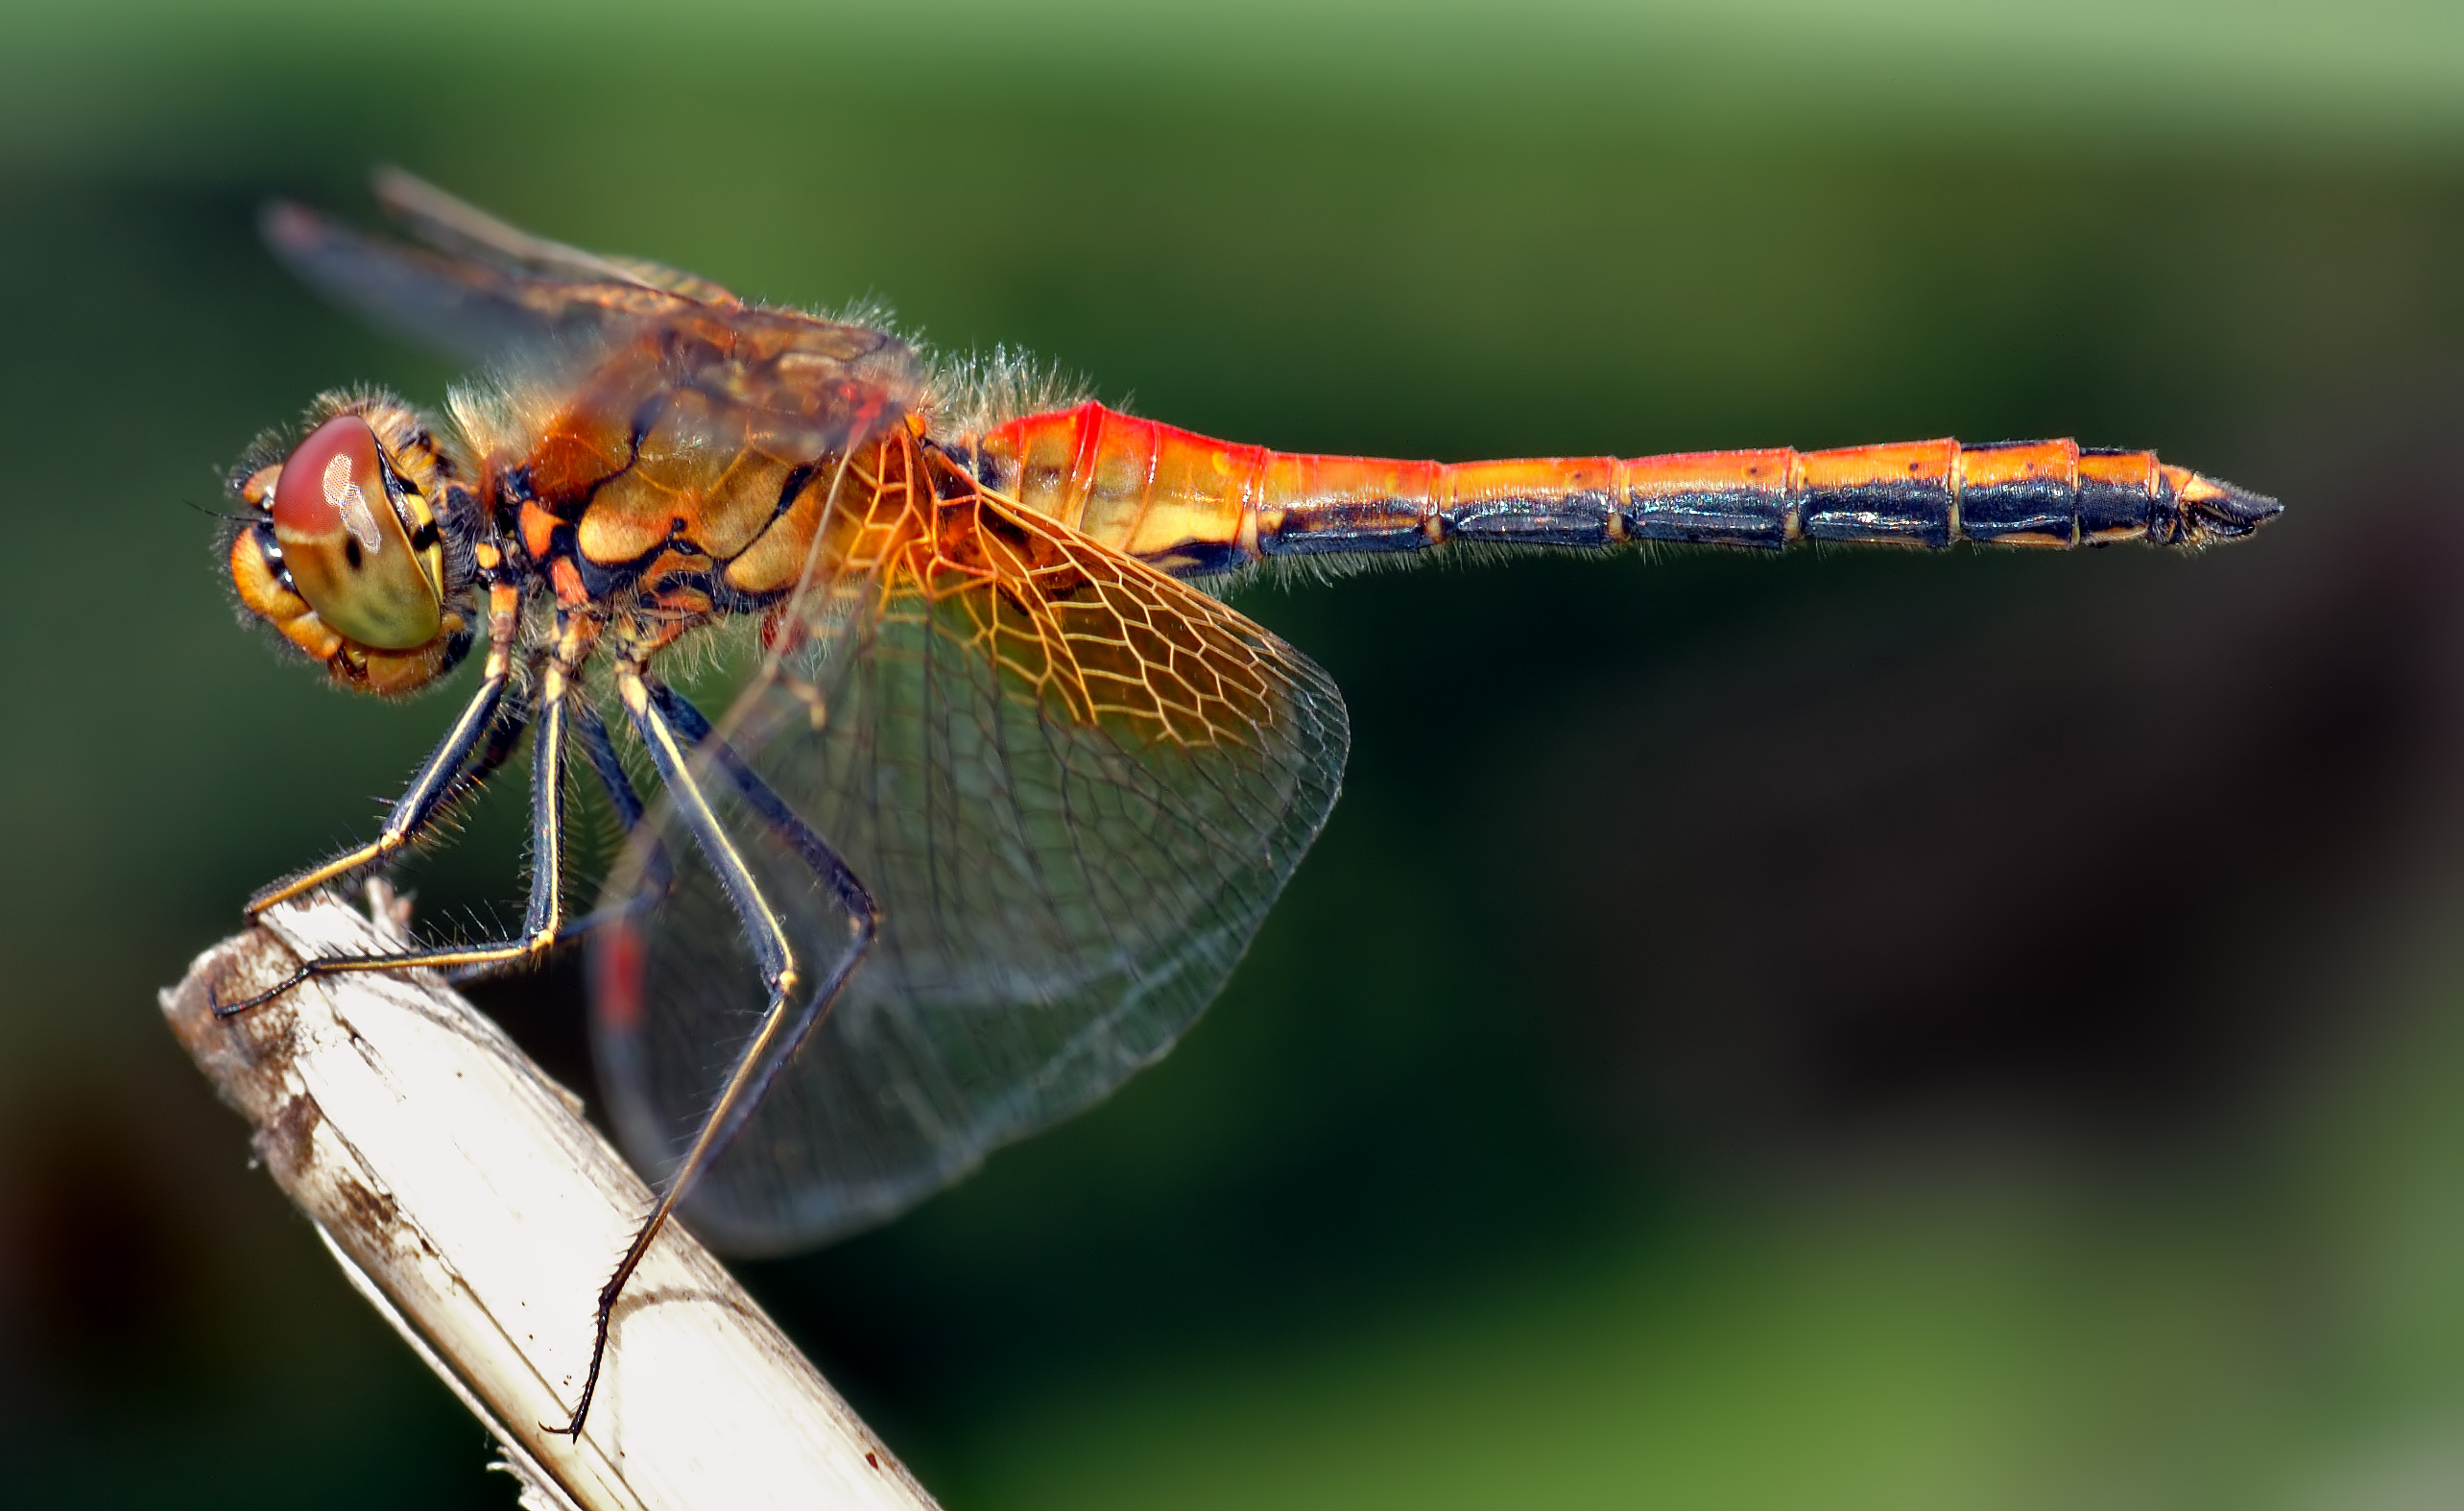
\includegraphics{assets/img/Sympetrum_flaveolum_-_side_(aka).jpg}
\caption{Zer eragiten dizu?\ldots{} eta zelan du izena?}
\end{figure}

\hypertarget{hizkuntza-sortzeko-tresna}{%
\section{Hizkuntza: sortzeko tresna}\label{hizkuntza-sortzeko-tresna}}

Hizkuntza bera ere sortzeko tresna bada. Hizkuntza erabili behar dugu adierazpenerako honakoak egiten ditugunean:

\begin{itemize}
\tightlist
\item
  Poemak
\item
  Ipuinak
\item
  kantak
\item
  Ahokorapiloak
\item
  Igarkizunak
\item
  Hitz-jokoak
\end{itemize}

Kulturalki zabalpen handikoak dira bertsolaritza edo errefrauak, esate baterako.

\begin{quote}
\emph{Ago ixiletik ez da ezer jakiten}
\end{quote}

Eta gaztelaniaz,

\begin{quote}
\emph{Hombre refranero, hombre majadero}
\end{quote}

\hypertarget{T1A1}{%
\section*{Lehenengo ariketa: Hausnarketa}\label{T1A1}}
\addcontentsline{toc}{section}{Lehenengo ariketa: Hausnarketa}

Hurrengo puntuak taldeko hausnarketa bat egiteko erabili behar dituzue, ikuspegi bikoitz batetik: norbanako legez eta Haur Hezkuntzako irakasle(gai) legez

\begin{itemize}
\tightlist
\item
  Gure hizkuntzei zein erabilera ematen diegu? (H1/H2/\ldots)\\
  Nahi duguna nahi dugun moduan adierazteko balio digu?
\item
  Irakasle gisa, zer garrantzia du ikasgelan hizkuntza aberatsa eta adierazkorra erabiltzea?
\item
  Zer egin dezakegu hizkuntza ``tutu triste'' bat balitz bezala erabili beharrean haren gaitasun guztiaz baliatzeko?
\item
  Eta HHko gelan zein neurritan ematen zaie aukera umeei hurrengoak egiteko?

  \begin{itemize}
  \tightlist
  \item
    Ideiak ahalik eta ondoen formulatzeko, haien ekintzak justifikatzeko, esperimentatzen dutenaz hausnartzeko eta arrazonatzeko, argumentatzeko, azalpenak emateko, planifikatzeko, kontatzeko\ldots{} ?
  \item
    Haien mundu emozionalarekin konektatu eta sentimenduak eta emozioak hitzez adierazteko, haietaz kontzientzia hartzeko, emozioak eta sentimenduak konpartitzeko?
  \item
    Hizkuntzarekin jolasteko, sortzeko eta gozatzeko?\\
    Irakasle gisa, zer-nolako esperientziak eskaini ahal dizkiogu ume guztiei hizkuntzaren erabilerari dagokionean?\\
    Zelan erabili dezakegu elkarrizketa?\\
    Zer-nolako estrategiak erabili ditzakegu?
  \end{itemize}
\end{itemize}

\hypertarget{eskolaren-eginkizuna-hizkuntza-arloan}{%
\section{Eskolaren eginkizuna hizkuntza arloan}\label{eskolaren-eginkizuna-hizkuntza-arloan}}

Ikasleen hizkuntza-komunikaziorako gaitasuna garatzen laguntzea, hizkuntza eraginkortasunez erabil dezaten euren bizitzako egoera eta behar guztietan.

\hypertarget{hizkuntza-hhko-curriculumean}{%
\section{Hizkuntza HHko curriculumean}\label{hizkuntza-hhko-curriculumean}}

Hizkuntza beste hizkuntzekin (musika-hizkuntza, gorputz- hizkuntza, arte-hizkuntza, \ldots) eremu bakarrean bilduta ulertzen izan da:

\begin{quote}
Hizkuntzak: komunikazioa eta adierazpena

Eremu horrek, haurrek, beste batzuen artean, honako gaitasun hauek eskuratzea du xede:

Hizkuntza horiez guztiez jabetzea pixkanaka, beharrak, lehentasunak, sentimenduak, esperientziak eta errealitatearen errepresentazioak adierazteko\\
Hizkuntza, ideiak eta sentimenduak adierazteko asmoz, komunikatzeko, irudikatzeko, ikasteko eta gozatzeko tresna gisa erabiltzea
\end{quote}

Eusko Jaurlaritzaren Legebiltzarra. (2009). 2/2009 Dekretua, urtarrilaren 20koa, Haur Hezkuntzako curriculuma zehaztu, eta Euskal Autonomia Erkidegoan ikaskuntza horiek ezartzen dituena. \emph{Euskal Herriko Agintaritzaren Aldizkaria}, 21(469), 1--41.

\hypertarget{aro-kritikoa}{%
\section{Aro kritikoa}\label{aro-kritikoa}}

Zer da?\\
Aro kritikoa bat da hizkuntza guztientzat?\\
Aro kritikoa bat da hizkuntza trebetasun (irakurmena, ahozkera, ulermena, etab.) guztientzat?\\
Aro kritikoaren ondoren, posible ote da hizkuntza bat besteek bezala eskuratzea?

\url{http://www.youtube.com/watch?v=R1vgUSTyPWk}

Selinkerren ustez (Selinker, 1972) beste hizkuntza batean arrakasta osoa lortzen da jatorrizko hiztun bat bezala bezain ongi hitz egiterakoan, ados?

Aro kritikoa

CPH, (\href{https://en.wikipedia.org/wiki/Critical_period_hypothesis}{Critical Period Hypothesis}): Penfield \& roberts (1959)

\begin{quote}
Burmuinean {[}\ldots{]} zauriak nozitu dituzten haurrak kapaz dira hizkuntza berriro ikasteko. Burmuinean antzeko zauriak izandako helduek, aitzitik, ez dute gauza bera egiterik. --Perales, 2004: 21
\end{quote}

Autore askok ikuskera desberdinak hartu dituzte gaiaren gainean, baina aro kritikoren bat askok identifikatu dute. Desberdin, baina identifikatu, horrela honela laburbil daitezke esanguratsuenak:

\begin{itemize}
\tightlist
\item
  Penfield \& Roberts (1959): 9 urte
\item
  Lenneberg (1967): pubertaroa
\item
  Krashen (1973): 5 urte
\end{itemize}

\hypertarget{T1A2}{%
\section*{Bigarren ariketa}\label{T1A2}}
\addcontentsline{toc}{section}{Bigarren ariketa}

Irakurri Barreña (1994) \href{https://zientzia.eus/artikuluak/chomskyren-arauak-eta-hizkuntz-jabekuntza/}{artikulua} eta erantzun dagozkion itemak (banaka).

\begin{enumerate}
\def\labelenumi{\arabic{enumi}.}
\tightlist
\item
  Zelan ulertzen dute sortzaileek delako Gramatika Unibertsala?
\item
  Zelan liteke gramatikaren eta sintaxiaren jabekuntza bideratzen duen ahalmena gizakiok genetikoki daukagula esatea?
\item
  Zein motatako hornia da giza hizkuntzaz jabetzea ahalbideratzen duena?
\item
  Baina zelan izan liteke haurrak bere ama-hizkuntzaz jabetzea, jasotzen duen hizkuntz esperientzia mugatua eta okerrez betea bada?
\item
  Zer da Gramatika Unibertsala?
\item
  Zertzuk dira hizkuntzaren parametroak? Adibideak eman.
\item
  Nola ikasten du haurrak hizkuntza? Entseiu / errakuntza? Hurrenkerarik bada?
\item
  Zein adinarekin hasten da haurra ergatiboa edo pluralaren komunztadura erabiltzen? Eta autozuzentzeko gaitasuna?
\item
  Zertan oinarritzen da hizkuntza jabekuntzaren garapena?
\end{enumerate}

Barreñaren testua \href{../beste/Barena/Barrena_1994_Chomskyren_arauak_eta_hizkuntz_jabekuntza.pdf}{azpimarratuta}

\hypertarget{T1E}{%
\section*{Erreferentziak}\label{T1E}}
\addcontentsline{toc}{section}{Erreferentziak}

Barreña, A. (1994, ekainak 1). Chomskyren arauak eta hizkuntz jabekuntza. \emph{Elhuyar aldizkaria}, 1994, 25--31.

Eusko Jaurlaritzaren Legebiltzarra. (2009). 2/2009 Dekretua, urtarrilaren 20koa, Haur Hezkuntzako curriculuma zehaztu, eta Euskal Autonomia Erkidegoan ikaskuntza horiek ezartzen dituena. \emph{Euskal Herriko Agintaritzaren Aldizkaria}, 21(469), 1--41.

Eusko Jaurlaritzaren Legebiltzarra. (2015). 237/2015 Dekretua, abenduaren 22koa, Haur Hezkuntzaren curriculuma zehaztu eta Euskal Autonomia Erkidegoan ezartzen duena. \emph{Euskal Herriko Agintaritzaren Aldizkaria}, 141. \url{http://www.euskadi.eus/bopv2/datos/2016/01/1600142e.pdf}

Gutierrez Mangado, M. J., \& Ezeizabarrena Segurola, M. J. (2022). \emph{Hotsetik hitzera Nola bereganatzen dute hizkuntza haur euskaldunek?} Erein Argitaletxea.

Marina, J. A. (1993). \emph{Teoría de la inteligencia creadora}. Editorial Anagrama.

Perales, J. (2004). Euskara helduaroan ikasteko motibazioa: Hainbat gogoeta. \emph{Uztaro: giza eta gizarte-zientzien aldizkaria}, 50, 23--43.

Wells, Gordon. (1988). \emph{Aprender a leer y escribir}. Laia.

\hypertarget{hizkuntzalaritza}{%
\chapter{Hizkuntzalaritza}\label{hizkuntzalaritza}}

Hizkuntzalaritzaren inguruko oinarri gutxien-gutxieneko batzuk ikusiko ditugu gai honetan, eduki batzuk ulertu behar baitira, egoki jarraitu ahal izateko ikasgaian.

Gai honetan aurrerapausoak emateko glosategia sortu beharko duzu, pausurik pausu eta zure adibideak jarriaz.

\hypertarget{zer-da-hizkuntzalaritza}{%
\section{Zer da Hizkuntzalaritza?}\label{zer-da-hizkuntzalaritza}}

\begin{itemize}
\tightlist
\item
  Hizkuntzak eta hauekin zerikusia dituzten fenomenoak aztertzen
  dituen zientzia.
\item
  Hizkuntzak sistema bat bezala funtzionatzen du. Sistema horren
  barruan fonetika eta fonologia, morfosintaxia, lexikologia,
  semantika, pragmatika daude.
\end{itemize}

Hizkuntzalaritza zientzia oso zabala da eta hainbat arlo ditu.
Hona hemen batzuk:

\begin{itemize}
\tightlist
\item
  Hizkuntzen jabekuntza
\item
  Hizkuntzalaritza antropologikoa
\item
  Soziolinguistika
\item
  Psikolinguistika
\item
  Neurolinguistika
\item
  Hizkuntzalaritza historikoa edo konparatua
\item
  Korpusaren hizkuntzalaritza
\item
  Hizkuntzalaritza konputazionala
\item
  Hizkuntzalaritza aplikatua
\item
  \ldots{}
\end{itemize}

\hypertarget{zer-izan-behar-dugu-kontuan-hizkuntza-bat-ikasterakoan}{%
\subsection{Zer izan behar dugu kontuan hizkuntza bat ikasterakoan?}\label{zer-izan-behar-dugu-kontuan-hizkuntza-bat-ikasterakoan}}

Eragiten duten elementuak asko direla esan ohi da, ikertuenak hauek dira:

\begin{itemize}
\tightlist
\item
  Arreta: askotan hizkuntza bat ikasten dugunean ez ditugu gauza
  asko kontuan izaten\ldots{} (klasean ariketa laburra)
\item
  Filtro afektiboak (motibazioa tartean)
\item
  Kanpoko eta barneko faktoreak\ldots{}
\end{itemize}

\hypertarget{zer-da-filtro-afektiboa}{%
\subsection{Zer da filtro afektiboa?}\label{zer-da-filtro-afektiboa}}

\begin{itemize}
\tightlist
\item
  Filtro afektiboa L2 jabekuntza/ikaste prozesua ulertzeko teoria bat da, eta L2 bat jabetzeko/ikasteko arrakasta edo hutsegitearekin lotutako aldagai emozionalak azaltzen ditu.
\item
  Filtro psikologiko ikustezina da eta L2 jabekuntza/ikaste prozesua erraztu edo oztopatu dezake.
\item
  Filtro afektiboa altua denean, ikasleak estresa, antsietatea edo konfiantza eza esperimentatu ahal ditu, eta honek L2 jabekuntza/ikaste prozesuaren arrakasta eragotzi dezake. Filtro afektiboa baxua denean L2 praktikatzeko eta ikasteko jarrera positiboa eta arriskutsu bat (beldur barik) errazten du.
\end{itemize}

\begin{quote}
\textbf{Hausnarketa}\\
(a) Filtro afektiboa kontuan hartuta, zer nolako esperientzia izan duzu beste hizkuntzak ikasterakoan?\\
(b) Zer egin dezakegu filtro afektiboa txikitzeko?
\end{quote}

\hypertarget{hizkuntzaren-atal-nagusiak}{%
\section{Hizkuntzaren atal nagusiak}\label{hizkuntzaren-atal-nagusiak}}

\begin{itemize}
\tightlist
\item
  Semantika
\item
  Pragmatika
\item
  Morfologia
\item
  Sintaxia
\item
  Fonetika
\item
  Fonologia
\item
  \ldots{}
\end{itemize}

\hypertarget{semantika-eta-pragmatika}{%
\subsection{Semantika eta Pragmatika}\label{semantika-eta-pragmatika}}

\hypertarget{semantika}{%
\subsubsection{Semantika}\label{semantika}}

Zeinu linguistikoen esanahiaz arduratzen den hizkuntzalaritzaren azpiatala da. Semantikak esanahi batzuek besteekin duten erlazioa aztertzen du, baita hitzek erreferenteekiko erlazioan dituzten esanahi-aldaketak ere.

\hypertarget{pragmatika}{%
\subsubsection{Pragmatika}\label{pragmatika}}

Hizkuntzaren erabilera zuzena aztertzen du, eta hizkuntza testuinguru zehatz batean aztertzen du.

\hypertarget{esate-baterako}{%
\subsubsection{Esate baterako}\label{esate-baterako}}

\begin{quote}
Lagun bat afaltzera gonbidatzen duzu, eta zure lagunak pastel bat
hartzen duenean zure alabak esaten dio:

\begin{quote}
\emph{Pastela jaten baduzu gehiago lodituko zara!}
\end{quote}

Zu lotsatuta zaude eta ezin duzu sinetsi alabak lagunari esan diona.
\end{quote}

Alabak esan duenak zentzua dauka: pastela jaten badugu, lodituko gara. Baina testuinguru soziala dela eta, amak interpretatzen du alabak lagunari lodi dagoela esan diola. Beraz, lehenengo esaldia, \emph{pastela jaten badugu, lodituko gara}, semantikari egiten dio erreferentzia, baina esaldiaren erabilera zuzena/desegokia kasu honetan, pragmatikari.

Zuk horren antzerako adibide bat aurkitu behar duzu, ahaleginez, bizi izandako zerbait kontatuaz.

\hypertarget{ariketa-glosarioa-semantika-eta-pragmatika}{%
\subsubsection{Ariketa: Glosarioa, semantika eta pragmatika}\label{ariketa-glosarioa-semantika-eta-pragmatika}}

Bilatu hurrengo kontzeptuen definizioa eta euskarazko adibideak aipatu:

\begin{itemize}
\tightlist
\item
  hiponimoa
\item
  hiperonimoa
\item
  sinonimoa
\item
  antonimoa
\item
  homonimoa
\end{itemize}

\hypertarget{morfologia-eta-sintaxia}{%
\subsection{Morfologia eta Sintaxia}\label{morfologia-eta-sintaxia}}

\begin{itemize}
\tightlist
\item
  Morfologiak hitzen barneko egitura aztertzen du.
\item
  Nola bereizten ditugu hitzak morfologikoki?
\item
  izenak, adjektiboak, aditzak, adberbioak, determinatzaileak, izenordainak,
  partikulak, aditz laguntzaileak, \ldots{}
  Aztertu hurrengo esaldia morfologikoki:
\end{itemize}

\begin{longtable}[]{@{}
  >{\centering\arraybackslash}p{(\columnwidth - 4\tabcolsep) * \real{0.4615}}
  >{\centering\arraybackslash}p{(\columnwidth - 4\tabcolsep) * \real{0.2692}}
  >{\centering\arraybackslash}p{(\columnwidth - 4\tabcolsep) * \real{0.2692}}@{}}
\toprule()
\begin{minipage}[b]{\linewidth}\centering
Lagunarekin
\end{minipage} & \begin{minipage}[b]{\linewidth}\centering
etorri
\end{minipage} & \begin{minipage}[b]{\linewidth}\centering
nintzen
\end{minipage} \\
\midrule()
\endhead
Lagun-a-rekin & etor(r)-i & n-in-tze-n \\
Izena-artik.det.-soziatiboa & aditz erroa-aspk. & 1.per-erro.asp-1.per-irg. \\
\bottomrule()
\end{longtable}

\hypertarget{euskararen-kasua}{%
\subsubsection{Euskararen kasua}\label{euskararen-kasua}}

Hitza maila goreneko unitatea da, morfema unitate minimoena.

Morfema gramatikalak: funtzio gramatikal eta sintaktikoa.

\begin{itemize}
\tightlist
\item
  deklinabidea, artikuluak, etab.
\item
  Morfema lexikalak: erro baten esanahia.
\item
  erro = \texttt{etxe}, \texttt{edalontzi}, \texttt{zoriontasun}, \ldots{}
\end{itemize}

Deklinabideak

\begin{itemize}
\tightlist
\item
  Izen-sintagma: kasu gramatikalak
\item
  Leku-denborazko kasuak
\end{itemize}

\hypertarget{kasu-gramatikalak}{%
\paragraph{Kasu gramatikalak}\label{kasu-gramatikalak}}

\begin{itemize}
\tightlist
\item
  absolutoa: \texttt{Ø}\\
  \emph{mutil bat dator}
\item
  partitiboa: \texttt{-rik}\\
  \emph{ez du dirurik}
\item
  ergatiboa: \texttt{-k}\\
  \emph{neskak jan du}
\item
  datiboa: \texttt{-i}\\
  \emph{amari eman diot}
\end{itemize}

\hypertarget{leku-denborazko-kasuak}{%
\paragraph{Leku-denborazko kasuak}\label{leku-denborazko-kasuak}}

\begin{itemize}
\tightlist
\item
  inesiboa: \texttt{-n}\\
  \emph{etxean}, \emph{amarengan}
\item
  leku-genitiboa: \texttt{-ko}/\texttt{-go}\\
  \emph{etxeko}
\item
  adlatiboa: \texttt{-tik}, \texttt{-ra}, \texttt{-rako}, \texttt{-raino}, \texttt{-rantz}\\
  \emph{etxetik}, \emph{amarengandik}; \emph{etxera}, \emph{amarengana}; \emph{etxerako}, \emph{amarenganako}; \emph{etxeraino}, \emph{amarenganaino}; \emph{etxerantz}, \emph{amarenganantz}
\end{itemize}

\hypertarget{beste-osagarri-batzuk}{%
\paragraph{Beste osagarri batzuk}\label{beste-osagarri-batzuk}}

\begin{itemize}
\tightlist
\item
  genitiboa: \texttt{-en}\\
  \emph{neskaren}
\item
  instrumentala: \texttt{-z}\\
  \emph{gazteleraz}
\item
  soziatiboa: \texttt{-kin}\\
  \emph{neskarekin}
\item
  motibatiboa: \texttt{-(n)gatik}\\
  \emph{neskagatik}
\item
  destinatiboa: \texttt{-entzat}\\
  \emph{neskarentzat}
\end{itemize}

\href{https://www.hiru.eus/eu/lengua-vasca/sintagmas-de-la-oracion-declinacion}{Gehitxuago jakiteko}

\hypertarget{ariketa-aztertu-hurrengo-esaldia-morfologikoki}{%
\subsubsection*{Ariketa: Aztertu hurrengo esaldia morfologikoki}\label{ariketa-aztertu-hurrengo-esaldia-morfologikoki}}
\addcontentsline{toc}{subsubsection}{Ariketa: Aztertu hurrengo esaldia morfologikoki}

Laguntza ariketa hau egiteko, \href{http://ixa2.si.ehu.es/demo/analisianali.jsp}{hemen}

\begin{itemize}
\tightlist
\item
  Amaren etxera noa.
\item
  Atzo ez ginen eskolara etorri.
\item
  Hemen salda dago.
\item
  Medikuarengana joan behar dut.
\end{itemize}

\hypertarget{sintaxia}{%
\subsubsection{Sintaxia}\label{sintaxia}}

Sintaxiak, berriz, perpausen barneko egitura eta egitura horiek
perpausan betetzen duten funtzioa.

\href{https://www.ehu.eus/seg/hizk/1/4}{Gehitxuago jakiteko}

\hypertarget{T2A2}{%
\subsubsection*{Ariketa: Glosarioa, morfologia eta sintaxia}\label{T2A2}}
\addcontentsline{toc}{subsubsection}{Ariketa: Glosarioa, morfologia eta sintaxia}

Bilatu hurrengo kontzeptuen definizioa eta adibideak aipatu:

\begin{itemize}
\tightlist
\item
  izen-sintagma
\item
  aditz-sintagma
\item
  ergatiboa
\item
  komunztadura
\item
  perpausa
\end{itemize}

\hypertarget{fonetika-eta-fonologia}{%
\subsection{Fonetika eta Fonologia}\label{fonetika-eta-fonologia}}

\hypertarget{fonologia}{%
\subsubsection{Fonologia}\label{fonologia}}

fonemak eta beraien funtzioa aztertzen dituen zientzia. Fonemak unitate linguistiko txikienak dira, ez daukate esanahirik eta abstraktuak dira.
Esanahiak bereizteko balio dute: adibidez, \emph{kopa} eta \emph{topa}. \texttt{/k/} eta \texttt{/t/} ez dute esanahirik, baina bi hitz hauek bereizteko balio dute.

\hypertarget{fonetika}{%
\subsubsection{Fonetika}\label{fonetika}}

Fonetikak soinuak/hotsak eta beraien ekoizpena aztertzen dituen zientzia da. Hau da, soinuak nola eratzen diren eta nola hautematen diren.
Hotsak fonemen errepresentazio materialak dira.

\href{https://upload.wikimedia.org/wikipedia/commons/9/92/International_Phonetic_Alphabet_translated_into_basque_Nazioarteko_alfabeto_fonetikoa_eu.pdf}{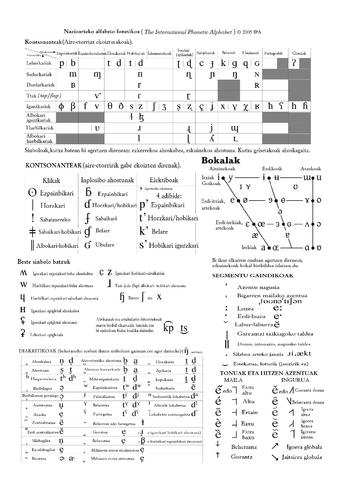
\includegraphics{assets/img/IPA(tx)_eu.pdf.jpg}}

\url{https://www.youtube.com/watch?v=gI6NaZRfnzU}

\url{https://www.youtube.com/watch?v=foImPuD_bKc}

\hypertarget{euskararen-hotsak}{%
\paragraph{Euskararen hotsak}\label{euskararen-hotsak}}

\hypertarget{bokalak}{%
\subparagraph{Bokalak}\label{bokalak}}

\texttt{/a/}
: erdiko bokal ireki edo behekoa

\texttt{/e/}
: aitzineko bokal erdi-ireki edo artekoa

\texttt{/i/}
: aitzineko bokal itxi edo goikoa

\texttt{/o/}
: atzeko bokal erdi-ireki edo artekoa

\texttt{/u/}
: atzeko bokal itxi edo goikoa

\texttt{/y/}
: aitzineko bokal biribildu itxi edo goikoa, ortografikoki \texttt{ü}z adierazten dena.

\hypertarget{kontsonanteak}{%
\subparagraph{Kontsonanteak}\label{kontsonanteak}}

24 fonema kontsonantiko daude. Fonemak honen arabera sailkatzen dira:

\begin{itemize}
\tightlist
\item
  ahots korden ekintza
\item
  sudur/aho barrunbearen arteko bereizketa
\item
  ahoskunea
\item
  ahots moldea
\end{itemize}

\hypertarget{T2A3}{%
\subsubsection*{Ariketa: Glosarioa, fonetika eta fonologia}\label{T2A3}}
\addcontentsline{toc}{subsubsection}{Ariketa: Glosarioa, fonetika eta fonologia}

Bilatu hurrengo kontzeptuen definizioa eta euskarazko adibideak aipatu:

\begin{itemize}
\tightlist
\item
  alofonoa
\item
  fonema
\item
  hiatoa
\item
  azentua
\item
  diptongo
\end{itemize}

\hypertarget{T2A4}{%
\section*{Ariketa nagusia}\label{T2A4}}
\addcontentsline{toc}{section}{Ariketa nagusia}

Marraztu hizkuntzaren elementuen jabekuntzaren hurrenkera; Barreña (2012) eta Garcia et all. (2014) erabiltzea duzu euskararako.

\hypertarget{T2A5}{%
\section*{Ariketa gehigarria}\label{T2A5}}
\addcontentsline{toc}{section}{Ariketa gehigarria}

Aurreko ikasturte batzuetan ariketa hau egin da kontzeptuak sendotze aldera. Ikasturte honetako egutegiagatik, aukeran dago egin ala ez:

\textbf{Euskara alderatu beste hizkuntza batekin} ezaugarri linguistikoetan oinarrituta.

\url{https://www.hiru.eus/eu/lengua/semantica} (09/10/2018)

\url{https://prezi.com/0s5igkyblus_/pragmatika/}

\url{https://www.euskadi.eus/web01-s2ing/eu/contenidos/articulo/c0301/eu_d0301008/0301008.html}

\url{https://ikasmaterialak.ehu.eus/hizkuntza-ikasketak/euskal-fonetika-fonologia/euskal-fonetika-fonologiaren-ikasketarako-gaiak.pdf}

\hypertarget{T2E}{%
\section*{Erreferentziak}\label{T2E}}
\addcontentsline{toc}{section}{Erreferentziak}

Barreña, A. (2012). Fonologiaren, lexikoaren, morfologiaren eta sintaxiaren garapena haur euskaldunengan. In \emph{Hizkuntzaz jabetzen} (0-6) (Libk. 16, or. 67--107). Mendebalde Kultura Alkartea.

Garcia, I., Barreña, A., Ezeizabarrena, M. J., Almgren, M., Arratibel, N., \& Barnes, J. (2014). Haur euskaldunen komunikazio-garapena neurtzen 30-50 hila-bete bitartean: MacArthur-Bates CDI-III tresnaren euskal bertsioa. \emph{Uztaro: giza eta gizarte-zientzien aldizkaria}, \emph{88}, 33--72.

Euskara Institutua, EHU. (2011). Hots motak, euskal soinuak. In \emph{Sareko Euskal Gramatika (SEG)}. \url{https://www.ehu.eus/seg/fon/1/1/1}

\hypertarget{nola-ikasten-du-umeak-hizketan}{%
\chapter{Nola ikasten du umeak hizketan?}\label{nola-ikasten-du-umeak-hizketan}}

Komunikazioaren garapena lehen urteetan etxean eta eskolan

Nola ikasten du umeak hitz egiten? Horixe da ikasgai honetako ardatza. Hori garatzeko hiru atal nagusi garatuko dira:

\begin{enumerate}
\def\labelenumi{\arabic{enumi}.}
\tightlist
\item
  Hizkuntza komunikatzeko tresna bezala. Hizkuntzaren jabekuntza eta garapena komunikazioaren markoan.
\item
  Umearen eta helduaren eginkizuna hizkuntzaren jabekuntza-prozesuan
\item
  Komunikazioaren garapena lehen urteetan.
\end{enumerate}

Horrela, ekin diezaiogun gaiaren lehenengo atalari:

\hypertarget{hizkuntza-komunikatzeko-tresna}{%
\section{Hizkuntza: Komunikatzeko tresna}\label{hizkuntza-komunikatzeko-tresna}}

Zer behar da hizkuntzak eraginkorki funtziona dezan? Hurrengo diagramak laburpena proposatzen du.

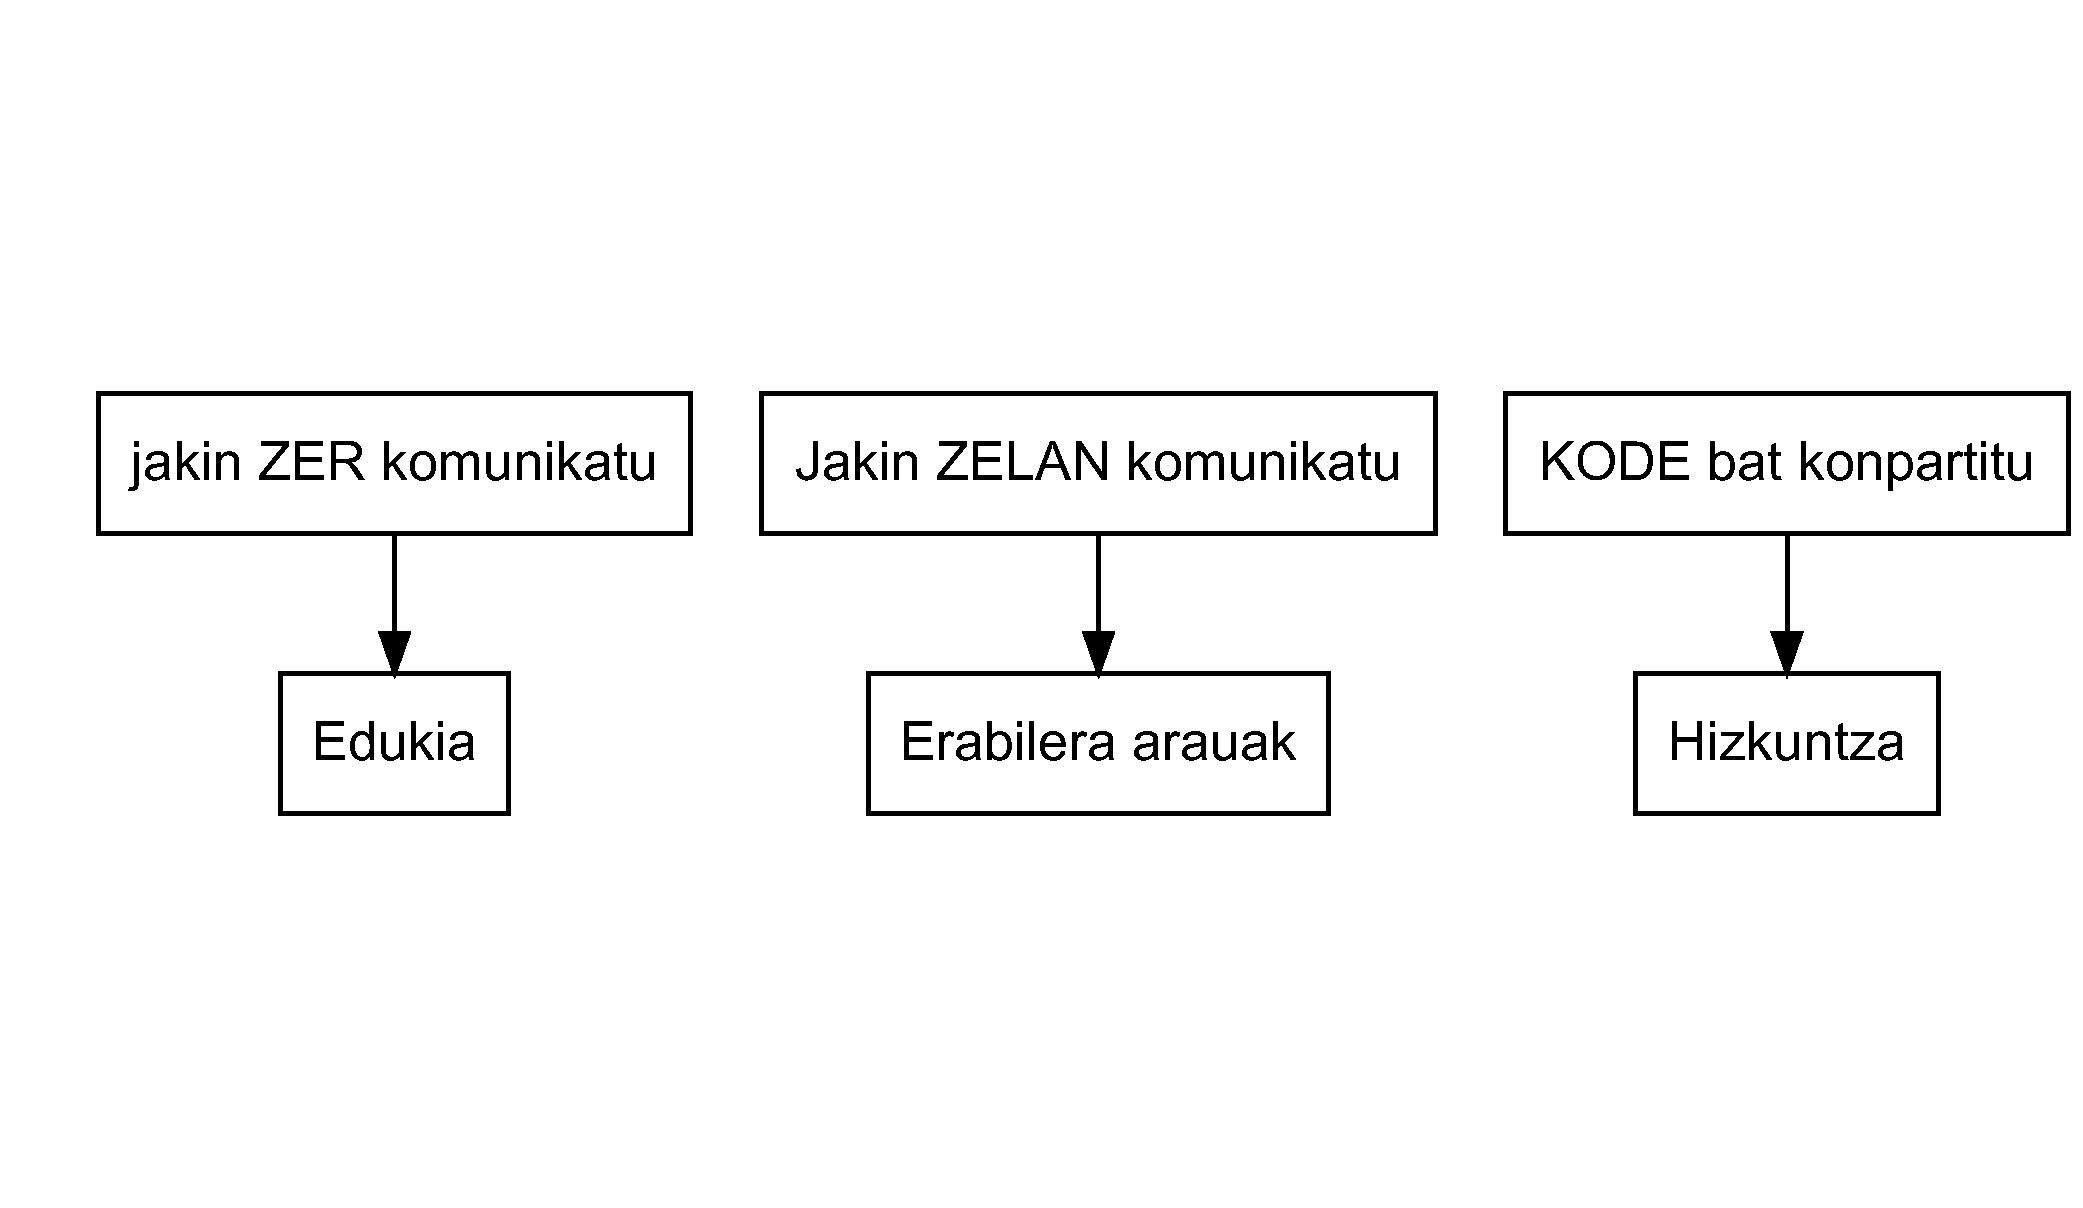
\includegraphics{Hizkuntzaren-Didaktikako-apunteak-V-0-HaurHezkuntza-2022_files/figure-latex/2.1-1.pdf}

Umeek horixe erabiltzen trebatzen dira holakoak eginaz:

\begin{itemize}
\tightlist
\item
  Besteekin elkarrekintzan arituz.
\item
  Euren inguruko pertsonekin askotariko jarduerak biziz eta partekatuz.
\item
  Umearen bilakaera-momentura egokituriko estrategiak erabiltzen dituzten helduekin ekinaz.
\end{itemize}

Berez, guretzat nabarmena izan daitekeen arren, kontuan izan behar dugu hizketan jardutea komunikazioarekin lotua dela, beraz, kontuan izatekoak dira hurrengoak, segidan garatuko ditugunak:

\begin{itemize}
\tightlist
\item
  Hizkuntzaren jabekuntza prozesua ez da lehenengo berbakin hasten, umearen komunikazioaren oinarriak ikastean hasten da
\item
  Berbaren agerrera prozesu horretan ulertu behar da, beharrizan zehatzei erantzunez sortuko den erantzun eraginkorra da hitza, hizkuntzaren garapeneko ernamuina
\item
  Hizkuntzaren jabekuntza eta garapena komunikazioaren markoan ulertu behar dira
\end{itemize}

\hypertarget{umearen-eta-helduaren-eginkizuna-hizkuntzaren-jabekuntza-prozesuan}{%
\section{Umearen eta helduaren eginkizuna hizkuntzaren jabekuntza-prozesuan}\label{umearen-eta-helduaren-eginkizuna-hizkuntzaren-jabekuntza-prozesuan}}

Tarte honek honako azpigaitan du banaketa

\begin{itemize}
\tightlist
\item
  Umeak eraikitzen du hizkuntza
\item
  Helduaren eginkizuna umeak egin behar duen eraikuntza horretan
\item
  Formatuak, helduon egingarrietako bat
\item
  Helduen umeekiko hizkuntzaren ezaugarri batzuk
\end{itemize}

\hypertarget{umearen-paper-aktiboa-hizkuntzaren-garapenean-umeak-eraiki-egiten-du-hizkuntza}{%
\subsection{Umearen paper aktiboa hizkuntzaren garapenean: umeak eraiki egiten du hizkuntza}\label{umearen-paper-aktiboa-hizkuntzaren-garapenean-umeak-eraiki-egiten-du-hizkuntza}}

\begin{itemize}
\tightlist
\item
  Umea, jaiotzen denetik, bere esperientzia interpretatzen saiatzen da. Horretarako dituen estrategiez baliatuko da, hasieran oso mugatuak izango direnak.
\item
  Umearen paper aktiboa hizkuntzaren garapenean: umeak eraiki egiten du hizkuntza.
\item
  Umeak nahiko antzera tratatuko ditu bere esperientziaren datu ezlinguistikoak eta datu linguistikoak:

  \begin{itemize}
  \tightlist
  \item
    Ezagutzaren beste arloetan bezala, umeak aurre egiten die komunikazioan sortzen zaizkion arazoei: material linguistikoa ere aztertzen du, inferentziak eta dedukzioak eginaz, oinarrizko legeak ateratzen eta hipotesiak egiten ditu. Ez du hartzen informazioa heltzen zaion bere horretan gordetzen: berreraiki egiten du, bere aurreezagutzetan oinarrituta.
  \item
    Aldez aurretik ezagutzen duena berrazterttzen du eta material \emph{ezagun} horrekin esperimentatzen du
  \end{itemize}
\end{itemize}

Lan hori egiteko, informazioa behar du hizkuntzaz eta hizkuntzaren erabileraz, informazio hori interpretatzeko estrategiak garatu eta aukeratu behar du hipotesiak nola egiaztatu.\\
Ume txikiaren interpretazio ahalmenak mugatuak direnez, ezinbestekoa da \textbf{helduak} haren \textbf{lana erraztea}.

\hypertarget{helduaren-eginkizuna-umearen-eraikuntza-lan-horretan}{%
\subsection{Helduaren eginkizuna umearen eraikuntza lan horretan}\label{helduaren-eginkizuna-umearen-eraikuntza-lan-horretan}}

Zergatik den aztertu barik, esan dezakegu lehen momentutik saiatzen dela heldua umearekin komunikatzen. Pentsa dezagun zer egiten dugun haur haioberri baten aurrean, eta gutariko gehienok (denok bagina, hobe) umeari hitz egiten diogu, berari, ez berari buruz; nahiz eta intelektualkti esango genukeen haurrak gure esanik ez lukeela ulertuko.

Helduak hori egiten duenean informazioa ematen dio umeari hizkuntzaz eta hizkuntzaren erabileraz harekin dituen harreman komunikatibo zuzenetan. Gainera, helduak umearen hipotesiak baieztatzen edo zuzentzen ditu.

Umearen lana errazten du helduak, andamiatu egiten du, haurraren gaitasunetara egokituta:

\begin{itemize}
\tightlist
\item
  hasieran behin eta berriz errepikatzen diren interakzio-marko egonkor eta mugatuak (formatoak) eskaintzen dizkio
\item
  ume txikiari zuzentzen dizkion hizkera eta esanahiak egokitzen ditu
\item
  beste estrategia batzuk ere bai
\end{itemize}

Helduak arreta berezia jartzen du entzule gisa umeak adierazten duena ondo ulertzeko, eta umeak esandakotik abiatuko da gaia garatuz edo umea bultzatuz berak egin dezan

\hypertarget{formatuak-andamiatze-mota}{%
\subsection{Formatuak: andamiatze mota}\label{formatuak-andamiatze-mota}}

Helduaren eta umearen arteko elkarrekintza patroiak dira, testuinguru mugatu, egonkor eta ezagunetan garatzen direnak.

Partaide bakoitzaren rolak zehaztuta daude formatuetan. Umea, formatuak menperatu ahala, helduarena izan den rol hura hartzen hasten da. Hasieran helduak kontrolatu eta zuzentzen du harremana.

Formatuak normalean umearen bizitzaren eguneroko errutinen inguruan erabiltzen ditugu, jana, loa, garbiketa, jolasa,\ldots{}

\hypertarget{formatu-motak}{%
\subsubsection{Formatu motak}\label{formatu-motak}}

\begin{description}
\item[Arreta bateratuko formatuak]
helduak eta haurrak une berean arreta objektu jakin batean jartzen duteneko interakzioak. (adibidez, irudi-liburuen irakurketa)
\item[Ekintza bateratuko formatuak]
heldua eta haurra objektu jakin batekin batera dabiltzaneko interakzioak. (adibidez, hartu-emoneko jolasak, sartu-aterakoak, eraikibotakoak,\ldots)
\end{description}

\textbf{Adibide bat}

Heldua eta haurra irudidun liburua irakurtzen

\begin{quote}
Zaintzailea (objektua seinalatuz) -: Begira

Haurra -: (\ldots)

Zaintzailea -: Zer da hori?

Haurra -: (\ldots)

Zaintzailea -: Txakurtxoa

Haurra -: (\ldots)

Zaintzailea -: Bai, txakurtxoa

Zaintzailea -: Nola egiten du txakurtxoak?

Haurra -: (\ldots)

Zaintzailea -: Uau, uau

Haurra -: Au

Zaintzailea -: Holaxe, bai, uau, uau
\end{quote}

\hypertarget{zertarako-formatua}{%
\subsubsection{Zertarako formatua:}\label{zertarako-formatua}}

Interpretazio marko gisa funtzionatzen dute. Formatuen erabileraren bitartez, umeari inguru ulergarriagoa eskaintzen diegu eta hor berak errazago hartuko du bere tokia eta eragiteko bidea.

\begin{itemize}
\tightlist
\item
  Umearentzat ulergarriagoa egiten dute haren inguruan gertatzen eta esaten dena (informazioa prozesatzeko umeak duen gaitasun mugatua kontuan hartu behar dugu)
\item
  Umearen parte-hartze aktiboa errazten dute (umeak egindakoak edota esandakoak erraz hartzen du esanahia testuinguru horretan).
\item
  Oinarrizko termino eta egitura linguistikoez hornitzen dute umea
\end{itemize}

\textbf{Adibide bat}: Helduak umearen diskurtsoa andamiatzen du

\begin{quote}
Ama -: Esan izekoari non egon zaren.

Umea -: Parke.

Ama -: Parkean, bai, parkean egon gara. Eta zer ikusi duzu? Esan izekoari zer ikusi duzun.

Umea -: Kua-kua.

Ama -: Ahatetxuak, ezta?

Umea -: Bai.
\end{quote}

\hypertarget{helduak-ume-txikiari-zuzentzen-dion-hizkeraren-ezaugarriak}{%
\subsection{Helduak ume txikiari zuzentzen dion hizkeraren ezaugarriak}\label{helduak-ume-txikiari-zuzentzen-dion-hizkeraren-ezaugarriak}}

Badira ezaugarri batzuk gizarte gehienetan aurki ditzakegunak:

\begin{itemize}
\tightlist
\item
  Hizkera enfatikoagoa: tonu altuak, goranzko intonazioa, azentu markatuagoak, keinuak, \ldots{}
\item
  Erritmo motelagoa
\item
  Hizkuntza-sistema erraztua:

  \begin{itemize}
  \tightlist
  \item
    artikulazio argia
  \item
    esaldi laburrak, sinpleak (sintaktikoki eta semantikoki) eta osoak
  \item
    ohiko lexikoa: konplexutasun eta dibertsitate gutxiagokoa\\
  \end{itemize}
\item
  ``Orain eta hemen''ari oso lotua
\item
  Galderazko, agintezko eta harridurazko perpausa ugari
\item
  Arreta lortzeko dei ugari
\item
  Errepikakorra
\item
  Hedatzeak (umeak esandakoa gramatikalki osatu edota semantikoki aberasten duten produkzioak)
\item
  \ldots{}
\end{itemize}

\hypertarget{komunikazioaren-garapena-lehen-urteetan}{%
\section{Komunikazioaren garapena lehen urteetan}\label{komunikazioaren-garapena-lehen-urteetan}}

Tarte nagusi bitan ulertu behar da oraingo atala, komunikazio aurrelinguistikoa eta komunikazio linguistikoa. Horrezaz gain, tarte bakoitza ere bitan zatitu behar dugu hobeto ulertzeko, hastapen momentuak eta garapen momentuak. Hala ere, kontuan izan behar dugu hain argi eta zehatz zatitzen duguna ideien planoan ez dela erraz mugatzen sarri.

\hypertarget{komunikazio-aurrelinguistikoa}{%
\subsection{Komunikazio aurrelinguistikoa}\label{komunikazio-aurrelinguistikoa}}

\hypertarget{hastapenak-0-4-hilabete}{%
\subsubsection{Hastapenak: 0-4 hilabete}\label{hastapenak-0-4-hilabete}}

\hypertarget{umeak}{%
\paragraph{Umeak}\label{umeak}}

\begin{itemize}
\tightlist
\item
  izaki aktiboa: bere inguruarekin harremanetan jarri eta interpretatuko du
\item
  inguruarekiko duen harremana ez homogeneoa: portaera ezberdinak pertsonekin eta objektuekin
\item
  berezkoa duen portaera-bagaiari esker (erreflexuak, biorritmoak, aurpegiekiko duten erakarpena, giza ahotsa beste soinuetatik bereizteko ahalmena, bokalizazioak\ldots), harreman sozial primitiboak helduarekin, portaera horiek intentziorik ez badute ere Komunikazio aurrelinguistikoaren hastapenak
\end{itemize}

\hypertarget{helduak}{%
\paragraph{Helduak}\label{helduak}}

\begin{itemize}
\tightlist
\item
  Lehenengo momentutik saiatzen da umearekin komunikatzen:

  \begin{itemize}
  \tightlist
  \item
    umearen portaerak intentzioz janzten ditu\\
  \item
    bere portaera umearenera egokitzen du: umearen mugimenduak, keinuak eta bokalizazioak berak egiten dituenekin txandakatzen saiatzen da (proto-elkarrizketa)\\
  \item
    interakzio-marko egonkor, mugatu eta errepikakorrak eskaintzen dizkio umeari, bera izanik bien arteko harremana kontrolatu eta zuzenduko duena (formatoak)
  \end{itemize}
\item
  Umearentzat oso gratifikanteak diren afektibitate adierazpenak erakusten dizkio
\end{itemize}

\hypertarget{garapena-5---12-hilabete}{%
\subsubsection{Garapena: 5 - 12 hilabete}\label{garapena-5---12-hilabete}}

\begin{itemize}
\tightlist
\item
  4-6 hilabeterekin, pertsonek ez ezik objektuek ere atentzioa emango diote umeari eta umea-heldua bikotea triangelu bihurtuko da\\
\item
  umeak portaeren balore komunikatiboa ikasiko du pixkanaka (``naturalki'' dituen portaerak ``kulturarki'' erabiltzen) eta keinuak, aurpegi-aiderazpenak, begiradak (batzuetan, bokalizazioez lagunduta) bere asmoak, desioak, interesak adierazteko erabiliko ditu
\item
  bokalizazioak gero eta gehiago hurbilduko dira inguruko hizkuntzaren soinuetara\\
\item
  urtearen bukaeran sortuko diren jolasak oso garrantzitsuak izango dira komunikazioaren garapenerako, elkarrizketaren arauak jarraitzen dituztelako (``jolas formatuak'' Bruner-en hitzetan)\\
\item
  afektibitateak jarraitzen du izaten haurrak komunikazioan egiten dituen aurrerapenen eragileetako bat
\end{itemize}

\hypertarget{jolasak-eta-komunikazioaren-garapena}{%
\subsubsection{Jolasak eta komunikazioaren garapena}\label{jolasak-eta-komunikazioaren-garapena}}

Urte bukaeran sortzen diren jolasek (hartu-emanekoek, sartu-aterakoek, eraiki-botakoek, kukuarenak,\ldots.) elkarrizketaren arauak jarraitzen dituzte.

Jolasteko:

\begin{itemize}
\tightlist
\item
  derrigorrezkoa da asmoa adierazten jakitea eta baita bestearen asmoa interpretatzen jakitea: \textbf{asmoaren iragarpena}
\item
  testuingurura erreferentziak egin behar dira: \textbf{Mekanismo deiktikoen erabilera}
\item
  gai bat konpartitzen ikasi behar da eta horren inguruan bariazioak egin: \textbf{Ustekizunak kontrolatzea}
\end{itemize}

\hypertarget{komunikazio-linguistikoaren}{%
\subsection{Komunikazio linguistikoaren}\label{komunikazio-linguistikoaren}}

\hypertarget{hastapenak-12-24-hilabete-keinutik-berbara}{%
\subsubsection{Hastapenak: 12-24 hilabete, keinutik berbara}\label{hastapenak-12-24-hilabete-keinutik-berbara}}

\begin{itemize}
\tightlist
\item
  Garapen biologiko eta kognitiboan aurrera egin ahala eta komunikazio esperientzia gehiago eta konplexuagoak dituen neurrian, umeak asmoak zehaztasun handiagoz eta modu ekonomikoago batez komunikatu nahi izaten ditu eta horrek berba erabiltzera bultzatzen du. Berbek hauek ordezkatzen dituzten keinuen funtzioak betetzen dituzte: eskatzea, eskaintzea, ukatzea, \ldots{}
\item
  Umearen lehenengo berbek ez dute helduentzat duten esanahi bera eta pixkanaka egokitzen joan behar izaten du helduek egiten duten erabilerara\\
\item
  Lehenengo urtearen bukaeran (18-24 hile) berbak funtzio berriak adierazteko erabiltzen ditu: informazioa eskatzeko, galderak erantzuteko, \ldots{}
\end{itemize}

\hypertarget{garapena-2-3-urte}{%
\subsubsection{Garapena: 2-3 urte}\label{garapena-2-3-urte}}

\begin{itemize}
\tightlist
\item
  Umearen hiztegia izugarri hazten da, kategoria gramatikal guztietako berbak erabiliko dituelarik (izenak, aditzak, izenordainak, adjektiboak, artikuluak, \ldots). Aditzak infinitiboan eta orain aldian\\
\item
  Hitzen lehenengo konbinazioak\\
\item
  Hiru urte betetzear dagoela, gai da mintzagaiari jarraitu eta hari informazioa gehitzeko, argitzeko eskaerak egingo ditu, \ldots{}
\end{itemize}

\hypertarget{urteko-umea}{%
\subsubsection{3 urteko umea}\label{urteko-umea}}

\begin{description}
\item[Sozialki]
Interakzioak izan ditzake hizkuntza erabiliz, elkarrizketaren oinarrizko arauak ezagutzen dituelako. Hala ere, interakzioaren arrakasta eta iraupena gaiaren eta solaskidearen trebetasunaren araberakoa izango da.
\item[Kognitiboki]
Bere mundua kategorizatu du eta gertaeren buru-errepresentazioak erabiltzen ditu gertakizun horietan parte hartzeko, gertatuko dena aurresateko eta gertatutakoa gogoratzeko.
\item[Linguistikoki]
Oinarrizko egitura linguistikoak eraiki ditzake bizi izandako gertakizunen berri emateko eta, inoren laguntzarekin, ordura arte partekatu ez duen informazioa emateko.
\end{description}

Hala eta guztiz ere, mintzagaian modu jarraituan eta helduek lagundurik aritzeak inplikatzen duen oso trebetasun mugatutik berdinekin eta informazio ez partekatuen inguruan erraztasunez aritu arte bide luzea geratzen da (M. Comadevall \& MC. Cardona).

\hypertarget{hhko-lehen-zikloko-irakasle-batek-kontuan-hartzekoa}{%
\subsection{HHko lehen zikloko irakasle batek kontuan hartzekoa}\label{hhko-lehen-zikloko-irakasle-batek-kontuan-hartzekoa}}

\begin{itemize}
\tightlist
\item
  Umeak trebetasun komunikatiboak besteekin era askotako egoeratan dituen harreman komunikatibo indibidualetan menperatzen ditu
\item
  Interakzio horietan eginbeharrekoa umearentzat motibagarria izan beharko da eta bere ahalmenetara egokitua, inplika dadin
\item
  Hasieran interakzioaren antolaketa helduaren esku egongo da
\item
  Afektibitatea haur txikiaren garapenaren eragile inportantea da
\end{itemize}

\hypertarget{urteko-umea-1}{%
\subsection{3-6 urteko umea}\label{urteko-umea-1}}

\begin{itemize}
\tightlist
\item
  Askotariko interakzio-testuingurutan hartzen du parte, asmo eta solaskide ezberdinekin, hizkuntzaren erabileran duen esperientzia zabalduz eta aberastuz. Berdinekiko interakzioak gero eta garrantzia handiagoa.
\item
  Garapen kognitiboan ere aurrerapen inportanteak garai honetan: 3 urterekin duen egozentrismoa gaindituz joango da, espazio eta denbora erlazioetan aurrera egingo du, gaitasuna lortuko du arrazoitze logikoak ulertzeko, gai izango da bere ezagutza kontzeptu berriekin erlazionatzeko, hizkuntza bere jarduera aurreratu eta antolatzeko erabiltzen ikasiko du\ldots{}
\item
  Hiztegia aberastuko du eta baliabide linguistiko berri asko eskuratuko ditu
\item
  Aurrerapen handiak hizkuntzaren erabilera kontestualizatuan eta lehenengo pausuak erabilera deskontestualizatuan

  \begin{itemize}
  \tightlist
  \item
    3 urterekin gaitasuna helduaren erabilera deskontestualizatua ulertzeko, gaiak sinpleak eta umearentzat erakargarriak direnean. Baina arazoak bere diskurtsoan ``hemen eta orain''a gainditzeko. Horretarako zailtasunak: a) oraindik egozentrismoa gainditu gabe; b) espazio-denborazko erlazioen menperatze-prozesuaren hastapenetan dago eta ezin du diskurtsoa horren arabera antolatu.
  \end{itemize}
\item
  4 urterekin ulertzen du helduaren diskurtso deskontestualizatuaeta trebatzen hasten da diskurtso deskontestualizatuetan. Egozentrismoa gainditzen. Gaitasuna oinarrizko espazio-denborazko erlazioak adierazteko eta aurrerapenak erlazio logikoen trebakuntzan ere, nahiz eta oraindik mugak izan erlazio horiek hitzez adierazteko.
\item
  5 urterekin gai da produkzio-testuinguruan presente ez dauden gauzez eta gertaerez hitz egiteko
\end{itemize}

\begin{longtable}[]{@{}
  >{\raggedright\arraybackslash}p{(\columnwidth - 2\tabcolsep) * \real{0.4949}}
  >{\raggedright\arraybackslash}p{(\columnwidth - 2\tabcolsep) * \real{0.5051}}@{}}
\toprule()
\begin{minipage}[b]{\linewidth}\raggedright
Erabilera kontestualizatua: produkzio-testuinguruaren menpe
\end{minipage} & \begin{minipage}[b]{\linewidth}\raggedright
Erabilera deskontestualizatua: produkzio-testuinguruarekiko dependentziarik ez
\end{minipage} \\
\midrule()
\endhead
Mezua adierazteko eta ulertzeko laguntza ez-linguistikoa Produkzio-testuinguruak informazioa ematen du Ez-hitzezko kodeak erabiltzen dira & Mezua adierazteko eta ulertzeko hitzetan oinarritu behar Produkzio-testuinguruak oso informazio gutxi Ez da ia erabiltzen ezhitzezko koderik \\
Esanahia zuzenean negoziatzeko aukera & Askotan aukerarik ez esanahia zuzenean negoziatzeko \\
Hiztegi eta egitura linguistiko arruntagoak & Hiztegi zehatza eta egitura linguistiko konplexuagoak \\
\bottomrule()
\end{longtable}

Hizkuntza umeak besteekin komunikatzeko duen tresna izatetik, bere buruarekin komunikatzeko tresna ere bihurtuko da, eta bere inguruan jarduten lagunduko dio umeari:

\begin{description}
\item[3 urte]
Hizkuntzak umearen jarduera laguntzen du, baina oraindik ez dio balio bera jarduera antolatzeko, planifikatzeko\ldots{} Hala ere, bere portaera eta besteena kontrolatzen laguntzen dio
\item[4 urte]
Hizkuntza ekintza aurreratzen eta antolatzen hasten da. Hizkuntza egozentrikoa.
\item[5 urte]
Hizkuntzak ekintza aurreratzen du eta jarduera planifikatzeko eta antolatzeko balioko dio
\end{description}

Besteek umearekin dituzten harremanetan hizkuntza asmo ezberdinetarako erabiliko dutenez, umea erabilera edo funtzio horietan trebatuz joango da.

Umeen hizkuntza funtzioak (J.TOUGH)

\hypertarget{hizkuntza-funtzioen-garapena}{%
\subsubsection{Hizkuntza funtzioen garapena}\label{hizkuntza-funtzioen-garapena}}

LEHENENGO: norberaren burua finkatu, gidatu, kontatu

GEROAGO: arrazoitu, iragarri, proiektatu, imajinatu

Funtzioen garapena kategoria bakoitzaren barnean ere gertatzen da:

\begin{itemize}
\item
  umeak funtzio horiek burutzeko erabiltzen dituen estrategia ezberdinek adieraziko dute garapenaren zein puntutan aurkitzen den, hau da, adierazten duen pentsamenduaren konplexutasun maila
\item
  Umeak hiztegia aberastu eta hizkuntzaren oinarrizko egiturak eskuratuko ditu.
\item
  Umearen berbetaren ezaugarri formalak:
\end{itemize}

\begin{description}
\item[3 urte]
L1eko fonema gehienen ahoskatzea

Izenordain posesiboen (1.2. perts), adjektiboen eta erakusleen erabilera

3-4 hitzeko esaldi sinpleak

trebetasuna baiezko eta ezezko adierazpen perpausen erabileran

aditzak indikatibozko orainaldian eta aginteran

aditzen aspektu burutuaren eta geroaren erabileraren hastapenak
\item[4 urte]
hiztegi zabala eta nahiko zehatza

pertsona izenordainen erabilera zuzena

perpaus konposatuen erabileraren hastapenak (koordinatuak, bereziki)

izenordain galdetzaileak galderetan

baldintzazkoen eta subjuntiboen erabileraren hastapenak
\item[5 urte]
L1en fonemen ahoskatze zuzena

hiztegi aberatsa

esaldi konposatuen (koordinatuak zein menpekoak) erabilera
\end{description}

\hypertarget{urteko-umea-2}{%
\subsection{5-6 urteko umea}\label{urteko-umea-2}}

\begin{description}
\item[Sozialki]
Besteekiko harreman mailak ahalbidetzen dio era koordinatuan jolastea eta jolasa hizkuntzaren bidez planifikatzea, nahiz eta oraindik gatazkak gerta daitezkeen. Berbeta solaskidearen beharrizanetara eta egoeretara egokitzen du.
\item[Kognitiboki]
Bere ezagutza kontzeptualaren barnean bere kultura propioaren hainbat ezagutza dago: landareak, animaliak, makinak, zenbakiak, espazioa, denbora. Gainera, ezagutza horrek ahalbidetzen dio azalpen luzeak jarraitzea, edukia ulertzea eta garrantzitsuak diren alderdiak gogoratzea.
\item[Linguistikoki]
5000-6000 berba inguruko hiztegia du, perpaus-egitura eta egitura diskurtsiboa ondo erabiltzen ditu eta talde sozialaren barruan erabilera oinarrizkoenak interpretatzeko beharrezkoa den hizkuntzaren erabilera pragmatikoa ulertzen du.
\end{description}

(M. COMADEVALL -- M.C.CARDONA)

\hypertarget{laburpena}{%
\section{Laburpena}\label{laburpena}}

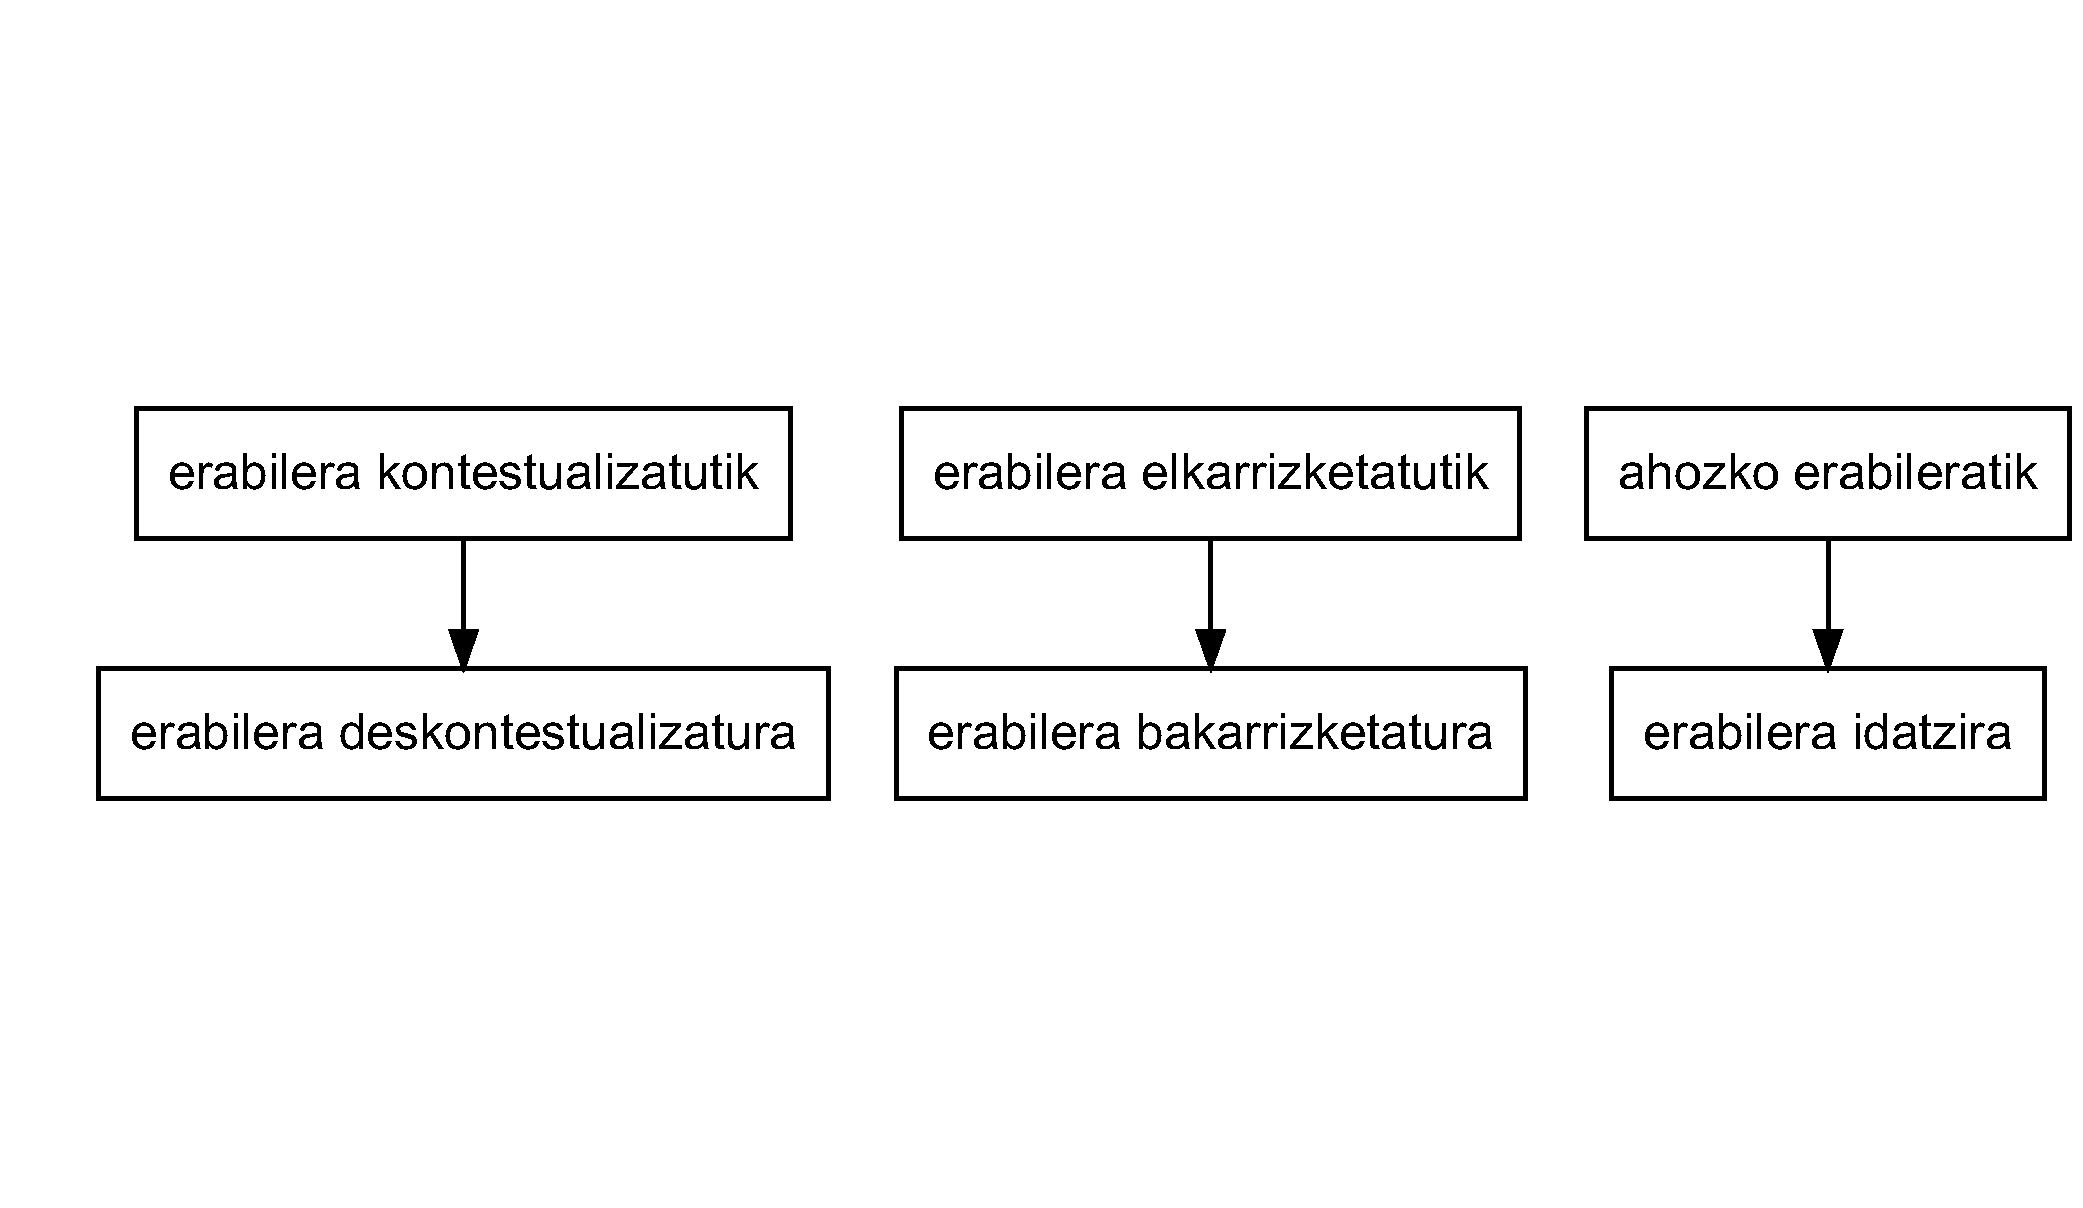
\includegraphics{Hizkuntzaren-Didaktikako-apunteak-V-0-HaurHezkuntza-2022_files/figure-latex/2.2-1.pdf}

\begin{longtable}[]{@{}
  >{\raggedright\arraybackslash}p{(\columnwidth - 2\tabcolsep) * \real{0.6118}}
  >{\raggedright\arraybackslash}p{(\columnwidth - 2\tabcolsep) * \real{0.3882}}@{}}
\toprule()
\begin{minipage}[b]{\linewidth}\raggedright
Hezitzaileak kontuan hartzeko
\end{minipage} & \begin{minipage}[b]{\linewidth}\raggedright
Egitekoak
\end{minipage} \\
\midrule()
\endhead
Haurrak komunikazio egoeratan parte hartuz ikasten du hitz egiten & Komunikazio egoerak sortu, antolatu \\
Hizkuntzaren funtzio ezberdinak garatzeko, umeak askotariko komunikazio egoeratan parte hartu behar du & Era askotako komunikazio egoerak sortu, antolatu \\
Behar-beharrezkoa umeak komunikazio egoeratan parte hartu nahi eta ahal izatea & Haurrarentzako esanguratsuak eta neurrikoak diren eginkizunak proposatu \\
Haurrak hizkuntzaren erabilera desberdinak elkarrizketetan ikasten ditu, berak baino gehiago dakien solaskide batekin & Elkarrizketa esperientzia aberatsak bultzatu \\
Elkarrizketa esperientziak onuragarriak izateko, helduak umeak esan nahi duena kontuan hartu eta haren ahalmen linguistiko eta kognitiboetara egokituko da & Elkarrizketetan, adi egon umeak esan nahi duenari eta egokitzapenak egin berbetan eta esanahietan \\
Ume txikiak trebetasun komunikatiboak besteekin dituen harreman komunikatibo zuzenetan menperatzen ditu & Ume bakoitzarekin harreman indibidualak bultzatu \\
Komunikazioan aurrera egiteko, oso inportanteak dira afektiboki gratifikanteak diren harremanak & Umeentzako afektiboki betegarriak diren harremanak bultzatu \\
\bottomrule()
\end{longtable}

\hypertarget{bibliografia}{%
\section{(Biblio)grafia}\label{bibliografia}}

Gehiago eta sakonago jakiteko, oso gomendagarria da hurrengo liburua, euskaran ardaztuta eta azalpen didaktiko ugari gaztelania zein frantsesarekin:

Gutierrez Mangado, M. J., \& Ezeizabarrena Segurola, M. J. (2022). \emph{Hotsetik hitzera Nola bereganatzen dute hizkuntza haur euskaldunek?} Erein Argitaletxea.

Eta bideoetan oso interesgarriak izan litezke hurrengo dokumentalok (ingelesez ekoitzitakoak):

Ellis Entertainment (Director). (2004). \emph{Baby Human}. \url{http://www.imdb.com/title/tt1414346/}

Hickman, D., Klein, L., Britain), C. F., Entertainment (Firm), R., Ltd, W. to W. T., \& Networks, D. (Directors). (1994). \emph{Baby it's you. Volume one, In the beginning., First steps}. {[}Australia{]}\,: Roadshow Entertainment. \url{https://trove.nla.gov.au/version/18675181}

Bideoon gaztelaniazko itzulpenak ere badira, euskarazkorik ez dut ezagutzen.

\hypertarget{proiektua}{%
\chapter*{Proiektua}\label{proiektua}}
\addcontentsline{toc}{chapter}{Proiektua}

Azalpenak \href{../beste/Proiektua/Deskribapena-dokumentua.pdf}{dokumentu honetan} eta orientabideak \href{../beste/Proiektua/Proiektua-Orientabideak_ahozko_aurkezpenerako.pdf}{ahozko aurkezpenerako hemen} eta \href{../beste/Proiektua/Proiektua-Orientabideak_idatzizko_lanerako.pdf}{idatzizkorako hemen}.

Transkripzioak egiteko \href{http://bosgarrena.blogspot.com/2019/10/transkripzioak-egiteko-erreminta-libre.html}{baliabide batzuei buruz} eta \href{../beste/Proiektua/senior_.html}{adibide bat} Transcriber softwarea \href{http://trans.sourceforge.net/en/presentation.php}{*} erabilita.

\hypertarget{baliabide-bibliografikoak}{%
\section*{Baliabide bibliografikoak}\label{baliabide-bibliografikoak}}
\addcontentsline{toc}{section}{Baliabide bibliografikoak}

Guibourg, I. (2000). El desarrollo de la comunicación. In Correig, M. \& Bigas, M. (arg.), \emph{Didáctica de la lengua en la educación infantil.} (orr. 13-42). Madrid: Síntesis.\\
\href{../beste/Proiektua/GUIBOURG_El_desarrollo_de_la_comunicacion.pdf}{Hemen}

Tough, J. (1996). \emph{El lenguaje oral en la escuela.} Madrid: Visor.\\
(3 testu)
\href{../beste/Proiektua/TOUGH_El\%20uso\%20del\%20lenguaje\%20en\%20los\%20ninos.pdf}{Hemen}, \href{../beste/Proiektua/TOUGH_como\%20hacer\%20una\%20valoracion\%20del\%20uso\%20del\%20lenguaje\%20en\%20el\%20nino.pdf}{hemen}, \href{../beste/Proiektua/TOUGH_utilizacion\%20de\%20los\%20cuadernillos\%20de\%20dibujos.pdf}{hemen} eta \href{../beste/Proiektua/TOUGH_Katutxo_beltza-irudiak.pdf}{\textbf{irudiak} hemen}.

\hypertarget{hizkuntza-patologiak}{%
\chapter{Hizkuntza patologiak}\label{hizkuntza-patologiak}}

Hizkuntza patologiei ere tarte bat eman behar zaio Haur Hezkuntzako graduko formakuntzan. Hala ere, ez dugu ahaztu behar formakuntzak ez duela bideratzen ez diagnostikorako ezta tratamendu espezialdurako. Hori ahaztu gabe, ikasgai honetako ardatza gelan egingo den lana izango da.

\hypertarget{ohar-batzuk}{%
\section{Ohar batzuk}\label{ohar-batzuk}}

Neurohizkuntzalaritza = Neurologia + Hizkuntzalaritza

Ikuspegi nagusi ditugu euren artean: Lokalizaziozionistak Vs Konexionistak

Garuna
Ideia hizkuntzara daramagu, garunean

Nerbio sistema:

\begin{itemize}
\tightlist
\item
  Zentrala
\item
  Periferikoa
  + Mintzamena
  + Idazmena
  + Keinu hizkuntzak
\end{itemize}

Hizkuntza Nahasmenak

\begin{longtable}[]{@{}
  >{\raggedright\arraybackslash}p{(\columnwidth - 4\tabcolsep) * \real{0.3659}}
  >{\raggedright\arraybackslash}p{(\columnwidth - 4\tabcolsep) * \real{0.3659}}
  >{\raggedright\arraybackslash}p{(\columnwidth - 4\tabcolsep) * \real{0.2683}}@{}}
\toprule()
\begin{minipage}[b]{\linewidth}\raggedright
Organikoa
\end{minipage} & \begin{minipage}[b]{\linewidth}\raggedright
Funtzionala
\end{minipage} & \begin{minipage}[b]{\linewidth}\raggedright
Bigarren mailakoa
\end{minipage} \\
\midrule()
\endhead
Afasia Anartria Alexia Agrafia Disfasia Disartria Hipoakusia & Hizkeraren atzerapen sinpleak Disfasia ebolutiboa Dislexia ebolutiboa Dislalia Disfemia Disfonia & Nahasmen deribatuak (THDA, epilepsia\ldots) \\
\bottomrule()
\end{longtable}

Apunte hauetan aberats.

\hypertarget{lana-hizkuntza-patologia-bat-haur-hezkuntzako-gelan}{%
\section{Lana: Hizkuntza patologia bat Haur Hezkuntzako gelan}\label{lana-hizkuntza-patologia-bat-haur-hezkuntzako-gelan}}

Ikasgelako talde bakoitzak lantzeko patologiaren bat aukeratu behar du eta holako pausuak eman behar dira horretan oinarrituta:

\begin{enumerate}
\def\labelenumi{\arabic{enumi}.}
\tightlist
\item
  Justifikatu aukera (irakaslea konbentzitu aukeraketaren mesedeaz)
\item
  Ikasi nahasmenduaren inguruan hurrengo ardatzak hartuta

  \begin{itemize}
  \tightlist
  \item
    Ezaugarriak (fisiologikoak, sozialak, portaerazkoak\ldots)
  \item
    Tratamenduak
  \item
    Haur Hezkuntzako gelan hartuko lituzkeen ezaugarriak.
  \item
    Haur Hezkuntzako irakasleak zer egin behar duen
  \end{itemize}
\item
  Gako kontzeptuak identifikatu
\item
  Prestatu diapositibak oharrekin
\item
  Talde guztiaren aurreko aurkezpena egin
\item
  Azterketa egin ikasitakoa ebaluatzeko
\item
  Txostena eman irakasleari (niri), azterketaren emaitzen hausnarketa bat duela.
\end{enumerate}

\hypertarget{derrigorrezko-bibliografia}{%
\section{Derrigorrezko bibliografia}\label{derrigorrezko-bibliografia}}

Derrigorrezko bakarra aipatzen zaizuen arren, zuen txostenetan aukeratzen duzuen lana egiteko baliabide egokiak hartuko dituzuela espero da.

Fernandez, B. (2012). \emph{Hizkuntza patologiak}.\\
\href{../Baliabideak/Fernandez-2012-hizkuntza-patologiak-eta-afasiak-garbi-.pdf}{Hemen}

\hypertarget{ahozko-hizkuntza-haur-hezkuntzan}{%
\chapter{Ahozko hizkuntza Haur Hezkuntzan}\label{ahozko-hizkuntza-haur-hezkuntzan}}

\begin{enumerate}
\def\labelenumi{\arabic{enumi}.}
\tightlist
\item
  Etxetik eskolara:\\
\end{enumerate}

\begin{itemize}
\tightlist
\item
  Etxea eta eskola ikas‐testuinguru ezberdinak
\item
  Eskolaren eskakizunak hizkuntza arloan
\end{itemize}

\begin{enumerate}
\def\labelenumi{\arabic{enumi}.}
\setcounter{enumi}{1}
\tightlist
\item
  Ahozko hizkuntza eta eskola:\\
\end{enumerate}

\begin{itemize}
\tightlist
\item
  Ahozkoa‐idatzia: ``continuum'' baten barruan
\item
  Ahozkoa vs ahozkoak. Ahozko kolokiala eta ahozko formala
\item
  Ahozko hizkuntzaren erabilerak eta funtzioak eskolan
\item
  Ahozkoa eskolan: ikasteko tresna eta ikasteko edukia
\end{itemize}

\begin{enumerate}
\def\labelenumi{\arabic{enumi}.}
\setcounter{enumi}{2}
\tightlist
\item
  Ahozko hizkuntza lantzeko orientabideak:\\
\end{enumerate}

\begin{itemize}
\tightlist
\item
  Hizkuntzaren garapenerako hezkuntza‐egoerak HHn
\item
  Espazioaren eta denboraren ntolaketa
\item
  Baliabideak eta estrategiak
\item
  Elkarrizketa
\end{itemize}

\hypertarget{etxetik-eskolara}{%
\section{Etxetik eskolara}\label{etxetik-eskolara}}

Etxea eta eskola testuinguru ezberdinak dira; nahiz eta batean zein bestean hizkuntza ikasten dugun inguruneen arteko aldeek baldintzatzen dituzte ikasteko aukerak eta bertan ikasitakoa ere bai.

\hypertarget{ezaugarriak}{%
\subsubsection{Ezaugarriak}\label{ezaugarriak}}

Etxean:

\begin{itemize}
\tightlist
\item
  banan banako interakzioa
\item
  ikaskuntza espontaneoa, ez da planifikatzen
\item
  gehienetan elkarrizketa eta ikaskuntza umeen interesetatik abiatzen dira eta helduekin burutzen dituzten jarduerei lotuta doaz / elkarrizketa‐gaiak umeen bizitzarekin lotura estua
\end{itemize}

Eskolan:
- irakaslea ume talde handi batekin / umeen arteko interakzioa
- ikaskuntza planifikatua
- umearen esperientzia eremua zabaltzen da: umeak ikasi behar du arreta gai edo jarduera batean jartzen eta arretari eusten eta ikasten duenak normalean ez du lotura zuzenik ikaskuntza gertatzen deneko testuinguruarekin
- Eskolaren eskakizunak hizkuntza arloan

Etxean:
- Haur guztiek eskuratzen dituzte oinarrizko baliabide linguistikoak eta lortzen dute trebetasuna ahozko erabilera elkarrizketatu eta kontestualizatuetan
- Haur batzuek harreman handiagoa kultura idatziarekin

Eskolak eskatzen ditu:
- trebetasuna hizkuntzaren erabilera deskontestualizatuan eta abstraktuan
- forma linguistiko konplexuen erabilera
- hiztegi espezifikoa ezagutzea, curriculumeko edukiekin erlazionatua
- umearen eguneroko esperientziatik urruntzen diren gaiak ulertu eta horien inguruan irakurtzea eta idaztea
- mezuaren hartzailea irudikatzea, aurrez aurre eduki beharrik gabe

\textbf{Hizkuntzaren erabileraren garapena gure gizarte alfabetatuan}

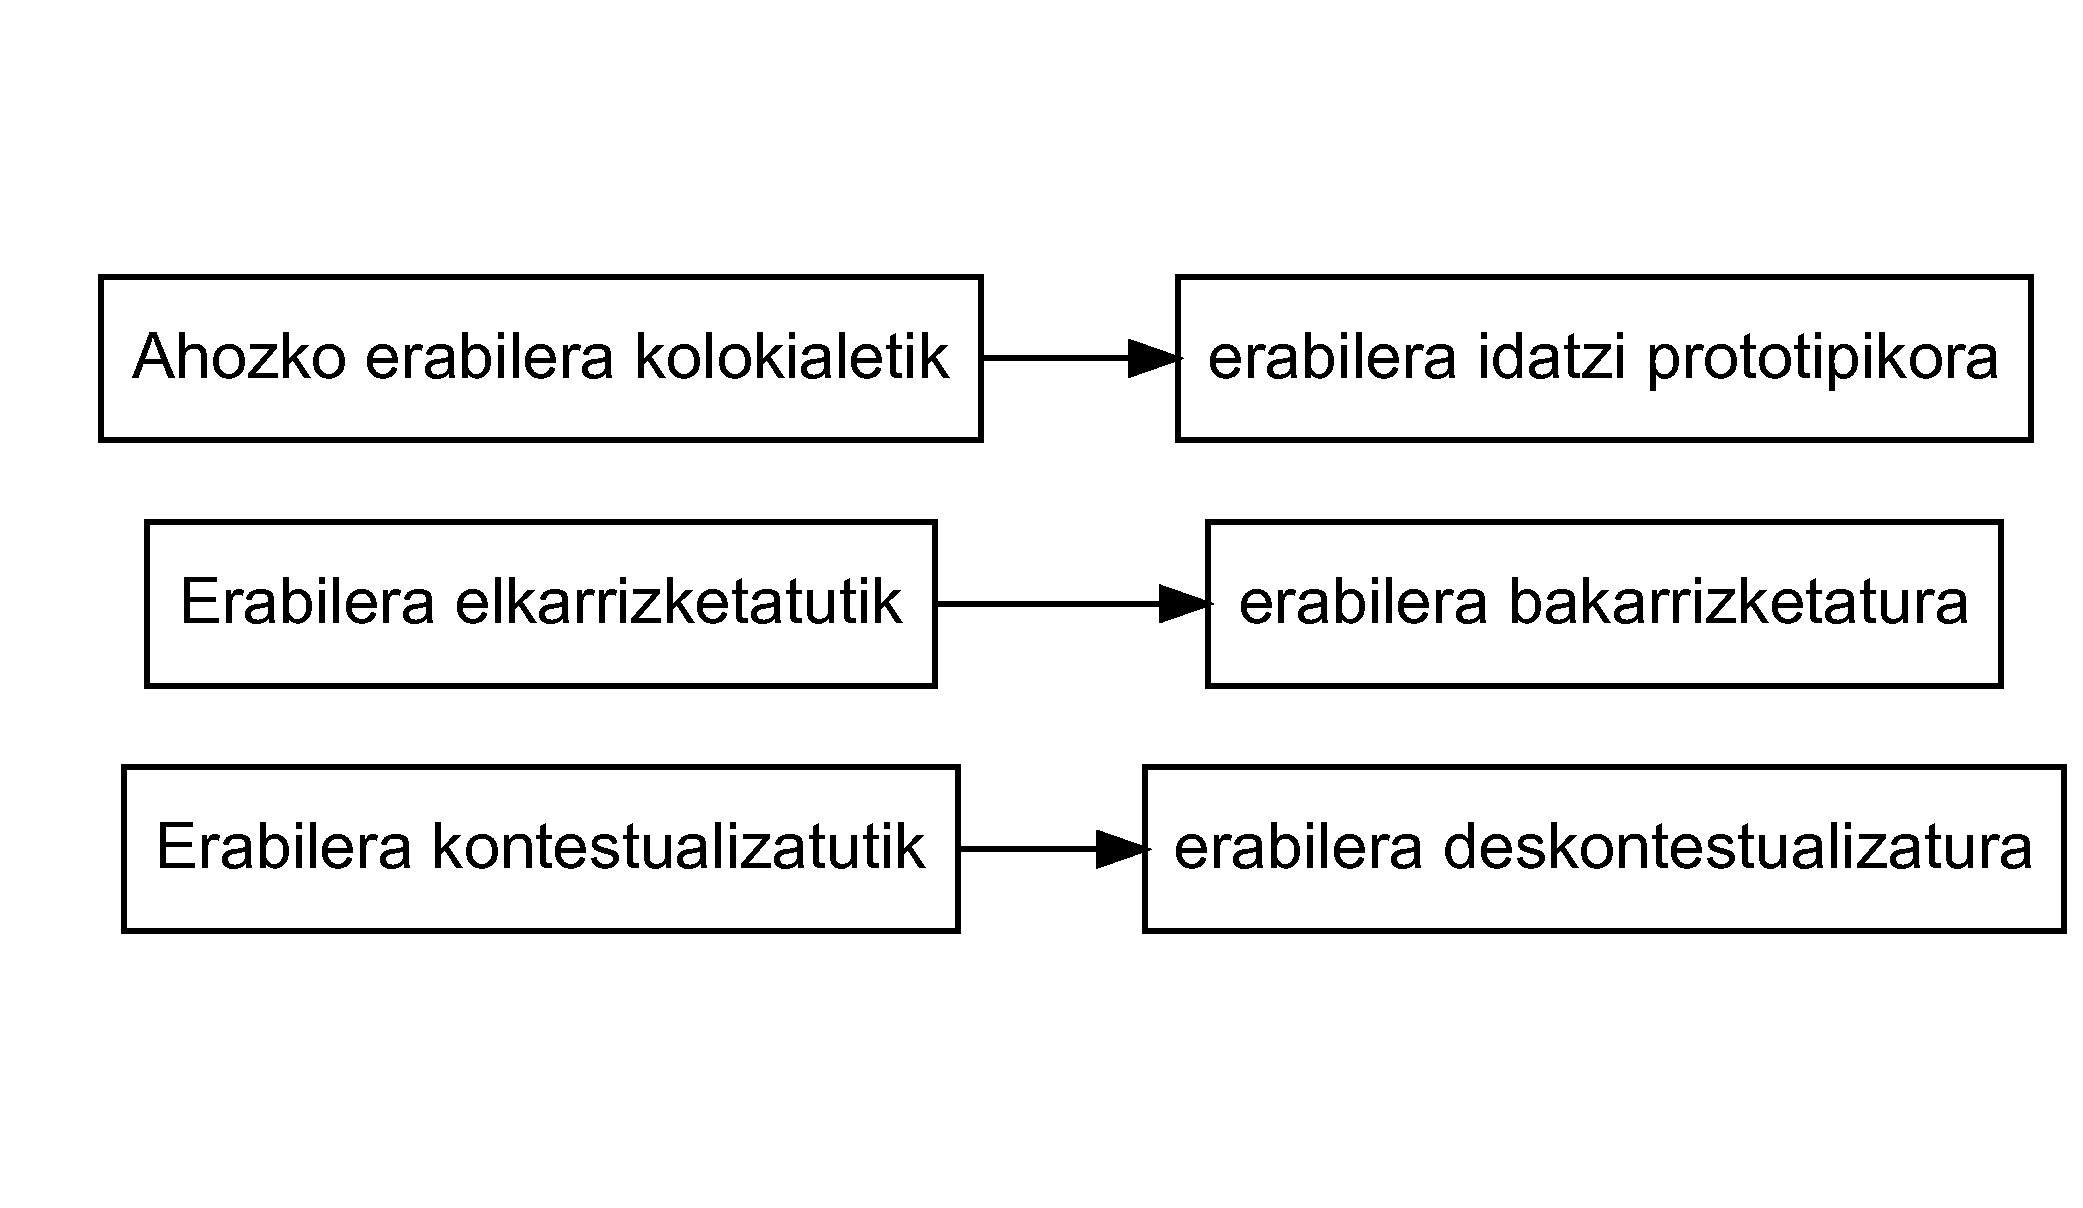
\includegraphics{Hizkuntzaren-Didaktikako-apunteak-V-0-HaurHezkuntza-2022_files/figure-latex/5.1-1.pdf}

\hypertarget{ahozko-hizkuntza-eta-eskola}{%
\section{Ahozko hizkuntza eta eskola}\label{ahozko-hizkuntza-eta-eskola}}

Ahozkoa \textasciitilde{} Idatzia: continuum batean

Askotan bereizten baditugu ere, bereizketa hori ez da erreala: gehienetan ahozkoaren eta idatziaren ezaugarriak dituzten testuak ekoizten ditugu (idatziaren ezaugarriak dituzten ahozko testuak, ahozkoaren ezaugarriak dituzten testu idatziak).

Komunikaziorako erabiltzen dugun kanalak berak (akustikoa/grafikoa) ez du guztiz erabakitzen testuen forma; badira-eta bestelako testuinguru-aldagai batzuk, eragin handiagoa dutenak (ikus hurrengo diapositibako koadroa).

Egokiagoa dirudi ``ahozko hizkuntza'' vs ``hizkuntza idatzia'' ikuspegi dikotomikoa gainditu eta ``continuum'' batez hitz egitea, ahozkoaren erabilera kontestualizatuenetik idatziaren erabilera deskontestualizatuenera doana

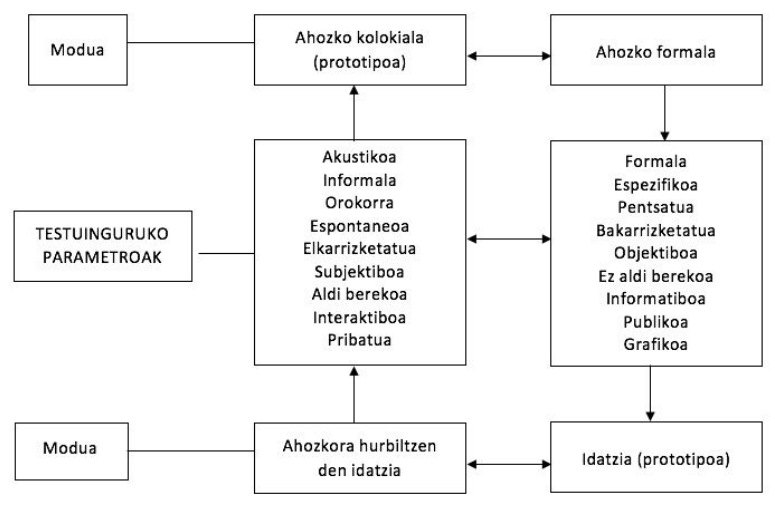
\includegraphics{assets/5-2.png}

\hypertarget{formaltasun-mailak}{%
\subsection{Formaltasun mailak}\label{formaltasun-mailak}}

\begin{longtable}[]{@{}
  >{\raggedright\arraybackslash}p{(\columnwidth - 2\tabcolsep) * \real{0.5000}}
  >{\raggedright\arraybackslash}p{(\columnwidth - 2\tabcolsep) * \real{0.5000}}@{}}
\toprule()
\begin{minipage}[b]{\linewidth}\raggedright
+
\end{minipage} & \begin{minipage}[b]{\linewidth}\raggedright
-
\end{minipage} \\
\midrule()
\endhead
- Espazio publikoa & - Espazio pribatua \\
- Harreman ierarkikoa & - Berdinen arteko harremana \\
- Gai espezializatua & - Eguneroko gaiak \\
- Planifikazio handiagoa & - Espontaneitate handiagoa \\
- Inpertsonala & - Inplikazio pertsonal handiagoa \\
- Zuzentasun formala & - Balizko akats formalak \\
- Lexiko teknikoa & - Lexiko zehaztugabea, egunerokoa \\
- Aldaera estandarraren erabilera & - Aldaera dialektalen erabilera \\
\bottomrule()
\end{longtable}

\textbf{Ahozko hizkuntza(k)}**

\emph{Ahozko hizkuntza} esaten diogun hori errealitate anitza da, ez da bat eta bakarra (erabilera kolokiala, harremanetarako hizkuntza / erabilera formala, akademikoa --idatziaren zenbait ezaugarri duena‐ )

Ahozko erabilera kolokiala modu naturalean garatzen da, baina ahozko formala garatzeko beharrezkoak dira entrenamendu sistematikoa eta hausnarketa, bereziki eskolan egiten direnak

Haur Hezkuntzan hasiko da \textbf{ahozko formalerako} hurbilketa garrantzitsua

Hizkuntza-erabilerak eskolan

\begin{itemize}
\tightlist
\item
  Harremanetarako hizkuntza (erabilera ez-formala)
\item
  Hizkuntza akademikoa (erabilera formala)
\end{itemize}

\begin{longtable}[]{@{}
  >{\raggedright\arraybackslash}p{(\columnwidth - 2\tabcolsep) * \real{0.5000}}
  >{\raggedright\arraybackslash}p{(\columnwidth - 2\tabcolsep) * \real{0.5000}}@{}}
\toprule()
\begin{minipage}[b]{\linewidth}\raggedright
Harremanetarako hizkuntza
\end{minipage} & \begin{minipage}[b]{\linewidth}\raggedright
Hizkuntza akademikoa
\end{minipage} \\
\midrule()
\endhead
- Etxean, kalean, modu espontaneoan garatzen da & - Eskolan ikasten da, modu sistematikoan \\
- Testuinguru ez‐linguistikoaren laguntza handia dauka & - Ez dauka testuinguru ez‐ linguistikoaren laguntzarik \\
- Esanahia negozia daiteke & - Esanahia testuan dago \\
- Sintaxia eta egitura linguistiko sinpleak & - Sintaxia eta egitura linguistiko konplexuak \\
- Lexiko ezaguna, arrunta & - Lexiko espezifikoa eta konplexua \\
- Kognitiboki eskakizun gutxikoa & - Kognitiboki eskakizun handikoa \\
\bottomrule()
\end{longtable}

\hypertarget{ahozko-hizkuntza-formala-haur-hezkuntzan}{%
\subsection{Ahozko hizkuntza formala Haur Hezkuntzan?}\label{ahozko-hizkuntza-formala-haur-hezkuntzan}}

Erregistro baten edo beste baten erabilera hizkuntzaz kanpoko faktoreek erabakitzen dute (non egiten dugun berba, norekin, zertaz,\ldots). Haur Hezkuntzako egoera:

\begin{itemize}
\tightlist
\item
  HHko ikasgela toki erabat publikoa ez bada ere (lortu nahi den hurbiltasun giroagatik), ez da familiarra edo pribatua: erdipublikoa da.
\item
  Irakaslearen eta ikasleen artean hierarkia dago, baina distantzia txikia (sortzen diren lotura afektiboak direla eta)
\item
  Gero eta gehiago, presente ez dagoenaz, umeen eguneroko esperientziatik urruntzen denaz, gai espezifikoagoez tratatzen da
\end{itemize}

Bestalde, HHn umeek hizkuntza idatziarekin dituzten harremanek (ipuinak, poemak, kantak, \ldots.) ahozko erabilera formalerako bidea zabaltzen diete

HHn, beraz, erabilera formalerako hurbilketa garrantzitsua

\hypertarget{zer-egin-haurrei-ahozko-formalaren-erabileran-laguntzeko-taldeko-elkarrizketetan}{%
\subsubsection{Zer egin haurrei ahozko formalaren erabileran laguntzeko taldeko elkarrizketetan?}\label{zer-egin-haurrei-ahozko-formalaren-erabileran-laguntzeko-taldeko-elkarrizketetan}}

\begin{itemize}
\tightlist
\item
  Anbiguotasuna eta zehaztasun falta gainditu dezaten, honakoak eskatu:
  azalpenak eta birformulazioak, erantzun esplizitoagoak, \ldots{}
\item
  Umeek beren adierazpenaren eta portaera komunikatiboaren kontzientzia hartzea sustatu
\item
  Ikasleen Ikasleen arteko solasaldia solasaldia bultzatu: bultzatu: hau da, korroan korroan normalean normalean erradiala erradiala izaten den interakziotik denen artekora pasatu
\item
  Irakasleak berak erabiltzeaz gain, umeei baliabide linguistikoak irakatsi

  \begin{itemize}
  \tightlist
  \item
    argibideak, errepikapenak, birformulazioak eskatu ditzaten (ez dizut ulertu, errepika dezakezu?, zer esan nahi du?,\ldots)
  \item
    beren interbentzioaren izaera modu argian agertu dezaten (ideiak azaltzeko, iritziak emateko --nik uste dut, nire iritzia esan nahi dut\ldots‐, proposamenak egiteko --nik uste \ldots egin beharko genukeela, proposamen bat egin nahi dut‐, \ldots{}
  \end{itemize}
\end{itemize}

\hypertarget{ahozko-hizkuntzaren-erabilerak-eta-funtzioak-eskolan}{%
\subsubsection{Ahozko hizkuntzaren erabilerak eta funtzioak eskolan}\label{ahozko-hizkuntzaren-erabilerak-eta-funtzioak-eskolan}}

\begin{itemize}
\tightlist
\item
  Hitz egitea eskolako bizitza soziala erregulatzeko, elkarrekin bizitzeko
\item
  Hitz egitea ikasteko ikasteko eta pentsatzen pentsatzen ikasteko ikasteko
\item
  Hitz egitea irakurtzeko eta idazteko
\item
  Hitz egitea hitz egiten ikasteko
\item
  Hitz egitea jolasteko, disfrutatzeko
\item
  Hitz egitea eskolako bizitza soziala erregulatzeko,
  elkarrekin bizitzeko

  \begin{itemize}
  \tightlist
  \item
    Berba eginez elkarrekin elkarrekin bizitzen bizitzen ere ikasten ikasten da
  \item
    Eskolako bizitza soziala erregulatzeko egiten den hizkuntzaren erabilera ikasteko iturri izan daiteke: askotan egoera formaletan egiten da berba eta horrek berba egiteko forma berriak ikastea dakar
  \end{itemize}
\item
  Hitz egitea ikasteko eta pentsatzen ikasteko

  \begin{itemize}
  \tightlist
  \item
    Elkarrizketa funtsezkoa da eskolako edukiak ikasteko: elkarrizketan ikasleak bere ideiak eta esperientziak azaltzen azaltzen ditu, besteenekin besteenekin konpartitu konpartitu eta alderatzen alderatzen ditu, esanahiak negoziatzen ditu, aurretik erabilitako argudioak eta arrazonamenduak berriro aztertu eta irakurketa berri bat egiten du\ldots.. Azken batean, ezagutza eraikitzen du
  \item
    Elkarrizketa funtsezkoa da jarrerei, baloreei\ldots{} buruz besteekin batera hausnartzeko
  \end{itemize}
\item
  Hitz egitea irakurtzeko eta idazteko

  \begin{itemize}
  \tightlist
  \item
    Irakurtzea ez da deszifratzea bakarrik. Batez ere, testuak ulertzea eta interpretatzea da, eta horretarako zenbait estrategia (inferentziak eta hipotesiak egin, informazio berria zaharrarekin erlazionatu, \ldots) garatu beharko ditu umeak. Trebatze horretan ahozko interakzioak garrantzia handia du
  \item
    Idaztea ez da kodifikatzea bakarrik. Batez ere, testuak ekoiztea da. Horretarako idatziko dena planifikatu eta ondoren idatzitakoa errebisatu beharko da. Planifikatzen eta idatzitakoa errebisatzen ahozko interakzioetan ikasten da
  \end{itemize}
\item
  Hitz egitea hitz egiten ikasteko

  \begin{itemize}
  \tightlist
  \item
    Ahozko erabilera formala ez da modu espontaneoan garatzen. Ikasi egin behar da solaskidearen beharrizanak kontuan hartzen, zehatza izaten, diskurtsoa modu autonomoan eraikitzen, \ldots{} Horretarako entrenamendua eta irakaskuntza sistematikoa behar da, ume txikien kasuan gehienbat elkarrizketaren bidez egingo dena.
  \end{itemize}
\end{itemize}

\begin{quote}
Ahozkoa eskolan:

\begin{itemize}
\tightlist
\item
  Ikasteko tresna
\item
  Ikasteko edukia
\end{itemize}
\end{quote}

\hypertarget{ahozko-hizkuntza-lantzeko-orientabideak}{%
\section{Ahozko hizkuntza lantzeko orientabideak}\label{ahozko-hizkuntza-lantzeko-orientabideak}}

Garatuko diren puntuak:

\begin{itemize}
\tightlist
\item
  Espazioaren eta denboraren antolaketa eta hizkuntzaren lanketa
\item
  Hizkuntzaren garapenerako hezkuntza-egoerak Haur Hezkuntzan
\item
  Irakaslearen baliabideak eta estrategiak umeari hizkuntzan eta pentsamenduan aurreratzen laguntzeko
\item
  Elkarrizketa
\end{itemize}

\hypertarget{espazioaren-eta-denboraren-antolaketa-eta-hizkuntzaren-lanketa}{%
\subsubsection{Espazioaren eta denboraren antolaketa eta hizkuntzaren lanketa}\label{espazioaren-eta-denboraren-antolaketa-eta-hizkuntzaren-lanketa}}

Bigas, M (2000)

\begin{itemize}
\tightlist
\item
  Umeak komunikazio-gaitasuna garatuko du hizkuntza erabiliz berarentzat esanguratsuak diren mota askotako jardueratan eta irakaslearen eta ikaskideen laguntzarekin. Zentzu horretan, gelako antolamenduak zeresan handia dauka garapen horretan.
\item
  Gelako antolamenduak ahalbidetuko ditu:

  \begin{itemize}
  \tightlist
  \item
    Komunikazio-egoera aberatsak eta umearentzat esanguratsuak
  \item
    Jarduera mota diferenteak, haurrak garatu beharreko hizkuntza-funtzioak lantzeko bidea emango dutenak

    \begin{itemize}
    \tightlist
    \item
      Proposatzen zaizkion zereginak burutzeko umeak hitz egin beharko du erabakiak hartzeko, hitz egin ekintzak antolatzeko edota ikaskideen portaeran eragiteko, hitz egin informazioa partekatzeko, arazoei irtenbideak bilatzeko, arrazoiak emateko, ideiak formulatzeko, denboran ordenatuak diren azalpenak emateko, erabakitakoaren inguruko argudioak emateko \ldots.
    \item
      Kontuan hartzeko: ahozko truke guztiek ez dute hizkuntzaren eta pentsamenduaren garapenean berdin eragiten
    \end{itemize}
  \item
    Taldekatze mota diferenteak, bai ikasleen arteko komunikazioa bai irakaslearen eta ikasleen artekoa sustatzeko bidea emango dutenak

    \begin{itemize}
    \tightlist
    \item
      Jolasean eta lanean aritzeko aukera anitzak eskaini : talde handia, talde txikiak, ikasleak bikoteka, irakaslea ikasle bakoitzarekin zuzenean, bakarka, \ldots{}
    \item
      Ikasleak taldeka jartze hutsak ez du, beste barik, komunikazio-gaitasunaren garapenean eta ikasketan laguntzen. Baldintza garrantzitsua da ikasleei proposatzen zaizkien eginkizunek haien arteko lankidetza eskatzea.
    \end{itemize}
  \end{itemize}
\end{itemize}

\hypertarget{hizkuntzaren-garapenerako-hezkuntza-egoerak}{%
\subsubsection{Hizkuntzaren garapenerako hezkuntza-egoerak}\label{hizkuntzaren-garapenerako-hezkuntza-egoerak}}

Egoerak antolatzeko orduan, kontuan izan:

\begin{itemize}
\tightlist
\item
  ikasgelako eguneroko bizitzaren inguruan sortzen direnak (sarrerak eta irteerak, egunaren hasierako eta bukaerako erritualak, jarduera aldaketa, hamarretakoa\ldots.)
\item
  Korroan eta txokoen inguruan sor daitezkeenak (elkarrizketa kolektiboa, ipuinen kontaketa eta antzezpena, jolas sinbolikoa -etxea, denda, \ldots-, arte plastikoa, esplorazio eta manipulazio jarduerak, jolasak, \ldots.)
\item
  Curriculumeko edukien inguruan sortzen direnak (gaiak eta gaien inguruan sor
  daitezkeen jarduerak eta proiektuak)
\item
  Ikastetxean bizi daitezkeen egoerak (patioko jolasak, eskolako jaia, jantokirako arauak adostea,\ldots)
\item
  Jarduera kulturalen inguruan sor daitezkeenak (Olentzero, Inauteriak,\ldots)
\end{itemize}

Hezkuntza-egoeren ekarpena umearen hizkuntzaren garapenerako egoeren ekarpena umearen hizkuntzaren garapenerako: landu daitezkeen alderdi linguistiko eta komunikatiboak (adibideak)

Direcció General d'Ordenació i Innovació Educativa, \& Departament d'Educació. (2004)

\begin{longtable}[]{@{}
  >{\raggedright\arraybackslash}p{(\columnwidth - 4\tabcolsep) * \real{0.3333}}
  >{\raggedright\arraybackslash}p{(\columnwidth - 4\tabcolsep) * \real{0.3333}}
  >{\raggedright\arraybackslash}p{(\columnwidth - 4\tabcolsep) * \real{0.3333}}@{}}
\toprule()
\begin{minipage}[b]{\linewidth}\raggedright
EDUKIA / NOZIOAK zertaz egiten den berba: munduaren ezagutza --semantika-
\end{minipage} & \begin{minipage}[b]{\linewidth}\raggedright
FORMAfonologia, morfologia, sintaxia, ..
\end{minipage} & \begin{minipage}[b]{\linewidth}\raggedright
ERABILERA/FUNTZIOAK zertarako egiten den berba
\end{minipage} \\
\midrule()
\endhead
- Jarduerari loturiko kontzeptuzko eta prozedurazko edukiak (antzezpena, gonbidapena eta oharrak, abestia, \ldots.) & - Kausa-ondorio harremanak adierazteko formak: -(e)lako -berokia janzten dugu hotz delako- & - Ekintza erregulatzea: jarduera antolatzea, laguntza eskatu eta eskaintzea, \ldots{} \\
- Lexikoa: jardueraren araberakoa & - Denbora harremanak adierazteko formak: lehenengo, gero, egun batean, \ldots. & - Informatzea: deskribatzea, azaltzea, kontatzea, sentimenduak eta emozioak adieraztea, \ldots{} \\
- Denbora eta espazio nozio eta harremanak, kausazkoak, ondoriozkoak, \ldots{} & - Ekintza adierazten duten aditzak: pintatu, moztu, \ldots. & - Hipotesiak egitea - Funtzio ludikoa (plazer hutsez abestea, adibidez) \\
& - Galderazko perpausak: zer \ldots?, nor \ldots.?, non \ldots? & - Eskertzeko/zoriontzeko formula sozialak praktikan jartzea \\
& - Hizkuntzaren alderdi suprasegmentalak: intonazioa, erritmoa & \\
& - Eskertzeko formulak: eskerrik asko, mila esker, \ldots{} & \\
\bottomrule()
\end{longtable}

\hypertarget{hh-klasean-lantzeko-adibide-bat}{%
\paragraph{HH klasean lantzeko adibide bat}\label{hh-klasean-lantzeko-adibide-bat}}

Gai bat aipatzen da klasean. Umeen artean eztabaidatzen dute zeri buruz ikasi nahi duten. Adibidez: HARTZA

\begin{itemize}
\tightlist
\item
  K-W-L taulak: zer dakigu? zer jakin nahi dugu? zer ikasi dugu?
\item
  Umeek hartzari buruzko informazioa biltzen dute: zer dakite hartzari buruz?
  Kartulina handi batean apuntatuko ditugu ideia guztiak.
\item
  Zer jakin nahi dute hartzari buruz? Informazioa bilatu behar dute.
  Adibidez: zer jaten du? non bizi da? zenbat pisatzen du?
\end{itemize}

Informazioa bilatzeko baliabideak:

\begin{itemize}
\tightlist
\item
  Elkarrizketak.
\item
  Liburuak: 3 hartzatxoen istorioa, Bavar eta Kiwi\ldots{} Heldu batek irakur dezake hartzekin zerikusia duen istorio bat klasean.
\item
  Non bizi dira hartzak? Mapamundia erabiliko dugu eta munduko hainbat leku ezberdinei buruz ikasiko dugu
\item
  Zer jaten dute? Naturari buruzko lanketa
\item
  Zenbat pisatzen/neurtzen du? Sistema metrikoa erabiliko dugu, matematikak\ldots{}
\end{itemize}

\hypertarget{hizkuntzaren-erabilera-jarduera-motari-lotua}{%
\paragraph{Hizkuntzaren erabilera jarduera motari lotua}\label{hizkuntzaren-erabilera-jarduera-motari-lotua}}

Arnau (1999)

\begin{longtable}[]{@{}
  >{\raggedright\arraybackslash}p{(\columnwidth - 2\tabcolsep) * \real{0.5000}}
  >{\raggedright\arraybackslash}p{(\columnwidth - 2\tabcolsep) * \real{0.5000}}@{}}
\toprule()
\begin{minipage}[b]{\linewidth}\raggedright
Jarduera ``akademikoak''
\end{minipage} & \begin{minipage}[b]{\linewidth}\raggedright
Jarduera ``sozialki esanguratsuak'':
\end{minipage} \\
\midrule()
\endhead
zentzuari garrantzirik ez (helburua: praktikatzea) & zentzuari garrantzia (asmo komunikatiboa) \\
trebetasun jakin batzuk garatzeko (adb.: zenbatzen ikasi) & askotariko trebetasunak garatzeko aukera (adb.: hitz egin, idatzi, irakurri, eduki matematikoak,\ldots) \\
interakzioak era batekoak (irakasleak gidatuta) & askotariko interakzioak (ikasleak rol aktiboagoa, ikasleen artekoak ere garrantzia) \\
Elkarrizketa irakasleak menperatzen du & Elkarrizketa orekatuagoa da \\
Ikasleak rol pasiboa du & Ikasleak iniziatiba handiagoa du \\
Ikasleak hizkuntza sinpleagoa erabiltzen du. Askotan, monosilaboak. & Hizkuntza asmo edo funtzio ezberdinetarako erabiltzen da \\
& Ikasleari hizkuntza konplexuagoa eta aberatsagoa erabiltzea eskatzen dio \\
\bottomrule()
\end{longtable}

\hypertarget{hizkuntzaren-garapenerako-hezkuntza-egoerak-1}{%
\subsubsection{Hizkuntzaren garapenerako hezkuntza-egoerak}\label{hizkuntzaren-garapenerako-hezkuntza-egoerak-1}}

Egoerak antolatzeko orduan, ez ahaztu:

\begin{itemize}
\tightlist
\item
  Umeak lehen pausoak emango dituela ahozko formalean eta erabilera hori ez dela modu naturalean garatzen
\item
  Hizkuntza ikasteko eta pentsatzeko tresna ere badela, eta ikasketan eta pentsamenduan aurrera egiteko elkarrizketa aberatsen premia dagoela
\item
  Ahozkoaren garrantzia hizkuntza idatzira hurbiltzeko (testu idatziak ulertzeko eta testu idatziak sortzeko)
\item
  Ahozkoak elkarbizitzarako duen balioa
\item
  Literatur baliabideen eta jolasen garrantzia umearen hizkuntzaren garapenerako
\end{itemize}

\hypertarget{elkarrizketa}{%
\subsubsection{Elkarrizketa}\label{elkarrizketa}}

Elkarrizketaren ekarpenak (Sánchez-Cano, 2009):

\begin{itemize}
\item
  Komunikazio trebetasunen garapenerako

  Elkarrizketan modu egokian aritzeko zenbait trebetasun lortu behar dira (elkarrizketan parte hartzea, denontzat berba egitea, \ldots), baina ez dira modu naturalean garatzen, entrenamendua eta hausnarketa eskatzen dute.
\item
  Alderdi linguistikoen garapenerako

  Elkarrizketak aukera ematen dio ikasleari berba egiteko, esaten dakienaz eta komunikatzeko dituen zailtasun linguistikoez kontzientzia hartzeko, esan eta segituan laguntza jasotzeko esandakoa hobeto adierazteko, alderdi linguistiko guztietan hobetzeko ( ahoskatzean eta intonazioan, morfosintaxian, lexikoan, diskurtsoaren eraikuntzan, \ldots)
\item
  Ikaskuntzarako baliabide gisa\\
  Irakaslearekin eta ikaskideekin hitz eginez ikasi ere egiten du ikasleak
\end{itemize}

Elkarrizketaren bidez, hitz egiten irakasteaz gain, lagundu ahal diegu umeei ``pentsatzeko eta ikasteko'' hizkuntza garatzen, estrategia ezberdinak erabiliz:

\begin{quote}
Gertaerak haien esperientzia eta emozio propioekin erlazionatzea ahalbidetuko dieten estrategiak

Prozesu kognitibo elaboratuagoak aktibatzera bideraturiko estrategiak

-- Comadevall, M (2012)
\end{quote}

\hypertarget{estrategia-batzuk}{%
\subsubsection{Estrategia batzuk}\label{estrategia-batzuk}}

\hypertarget{gertaerak-haien-esperientzia-eta-emozio-propioekin-erlazionatzea-ahalbidetzeko}{%
\paragraph{Gertaerak haien esperientzia eta emozio propioekin erlazionatzea ahalbidetzeko}\label{gertaerak-haien-esperientzia-eta-emozio-propioekin-erlazionatzea-ahalbidetzeko}}

Ipuinaren inguruko elkarrizketetan, elkarrizketa kolektiboetan edo antzeko egoeratan,
galderak edo iruzkinak egin \ldots{}

\begin{itemize}
\tightlist
\item
  Gertatzen dena (ipuinean edo ikaskideak azaltzen duena) haien esperientzia propioekin erlazionatzea ahalbidetzeko (gertatu zaizu inoiz zuri?, ikusi duzu inoiz\ldots.) . Helduak lagundu dezake bere esperientzia propioak azalduz ere.
\item
  Kausa-ondorio erlazioak ezartzea errazteko (zergatik?) edo erlazio horiek ezartzen direneko ereduak eman (uste dut hori egiteko arrazoia izan dela \ldots.).
\item
  Besteen emozioak eta sentimenduak ulertzen laguntzeko. Abiapuntua norberaren emozio eta sentimenduak komentatzea izan daiteke (zelan uste duzu sentituko dela printzesa?), edo irakaslearen komentarioak (minduta dago lagunak gezurra esan diolako, ni ere mintzen naiz hori gertatzen zaidanean).
\item
  Hartzen diren erabakien inguruan argudiatzea errazteko (hartu den erabaki bat egokia izan den ala ez, erabaki bera hartuko zenukeen ala ez, \ldots.)
\end{itemize}

\hypertarget{prozesu-kognitibo-elaboratuagoak-aktibatzera-bideratutakoak}{%
\paragraph{Prozesu kognitibo elaboratuagoak aktibatzera bideratutakoak}\label{prozesu-kognitibo-elaboratuagoak-aktibatzera-bideratutakoak}}

Galderak edo iruzkinak egin \ldots{}

\begin{itemize}
\tightlist
\item
  Gertatuko denaz hipotesiak eta iragarpenak egiten laguntzeko, umeen ezagutza eta esperientzietatik abiatuta (zer uste duzu gertatuko dela?, zer pasatuko litzateke\ldots.). Edo ereduak eman (nik uste dut gero \ldots..) .
\item
  (istorioan) azaltzen diren gatazkei edo arazoei irtenbideak bilatzen laguntzeko (zer egin genezake hori konpontzeko?, zein izango litzateke modurik hoberena \ldots?).
\item
  Besteen tokian jarri eta haien perspektiba hartzen laguntzeko (nola uste duzu sentitzen dela orain?), edo esperimentatu ez diren egoeratan jartzeko (politikaria izan nahi zenuke? zergatik?).
\item
  Antzezpenaren bidez praktikan jartzen lagundu ( istorioen antzezpenek, adibidez, laguntzen dute hari narratiboa eta pertsonaien sentimenduak eta emozioak ulertzen, eta pertsonaia horien perspektiba hartzen. Antzezpenaren planifikazioak, bestalde, irtenbideak aurkitzea, hipotesiak egitea, ebaluatzea \ldots. dakar)
\end{itemize}

\hypertarget{ariketa}{%
\section*{Ariketa}\label{ariketa}}
\addcontentsline{toc}{section}{Ariketa}

\href{../Baliabideak/05_ahozko_hizkuntza/Ahozkoa_eskolan-Lantzekoak.pdf}{Baliabideak}

\hypertarget{bibliografia-eta-erreferentziak}{%
\section*{Bibliografia eta erreferentziak}\label{bibliografia-eta-erreferentziak}}
\addcontentsline{toc}{section}{Bibliografia eta erreferentziak}

Arnau, J. (1999). Aproximaciones pedagógicas en la enseñanza de una segunda lengua a través de las matemáticas en la inmersión temprana. \emph{Journal for the Study of Education and Development, Infancia y Aprendizaje}, \emph{86}, 41--56.

Bigas, M. (2000). El lenguaje oral en la escuela infantil. In Correig, M. \& Bigas, M. (Eds.), \emph{Didáctica de la Lengua en la Educación Infantil} (pp.44-70). Madrid: Síntesis.

Camps, A. (2005). Hablar en clase, aprender lengua. In \emph{Hablar en clase: Cómo trabajar la lengua oral en el centro escolar} (or. 37--44).

Direcció General d'Ordenació i Innovació Educativa, \& Departament d'Educació. (2004). \emph{L'ús del llenguatge a l'escola: Propostes d'intervenció per a l'alumnat amb dificultats de comunicació i llenguatge}. Departament d'Educació, Servei de Difusió i Publicacions. \url{http://ensenyament.gencat.cat/web/.content/home/departament/publicacions/monografies/us-llenguatge-escola/lus_llenguatge_lescola.pdf}

Equipo de educación infantil y primer ciclo de primaria del CP Antzuola. (2010). Niños y niñas investigadores: ¿de qué hablamos? In \emph{Los proyectos de trabajo en el aula: Reflexiones y experiencias prácticas} (or. 29--42). Graó.

Sanchez-Cano, M., Cabra, M., Comallonga, L., Escudé, N., Font, E., Forés, N., Fuster, M., Giné, M., Grau, R., Mas, T., \& Ribó, E. (2009). \emph{La conversación en pequeños grupos en el aula}. Graó.

\hypertarget{murgiltze-klaseak-zer-izan-behar-dugu-kontuan}{%
\chapter{\texorpdfstring{Murgiltze klaseak Zer izan behar dugu kontuan?}{Murgiltze klaseak  Zer izan behar dugu kontuan?}}\label{murgiltze-klaseak-zer-izan-behar-dugu-kontuan}}

Hizkuntza ofizial bi: Euskara eta gaztelania\ldots{}

Hezkuntza sistemak Euskal Herrian elebitasuna oinarri:\\
Helburua : Bi hizkuntzak ezagutzea

Nola sustatu bi hizkuntzen ikaste prozesua?\\
Programa asko dago, hizkuntza biak hartzen dituzte kontuan.

Lau programa mota:

\begin{itemize}
\tightlist
\item
  Segregazioa
\item
  Sumertsioa
\item
  Mantentzea
\item
  Murgilketa
\end{itemize}

\hypertarget{segregazio-programak}{%
\section{Segregazio programak}\label{segregazio-programak}}

\begin{itemize}
\tightlist
\item
  Ikasleen L1 erabiltzen da eta L2 ikasgaitzat
\item
  Ikasleek L2n maila noa lortzen dutenean L2n eskolatzeko aukera ikusten da

  \begin{itemize}
  \tightlist
  \item
    Azken hori ia ez da gertatzen eta emaitza akademiko pobreak
  \end{itemize}
\item
  Ondorio negatiboak:

  \begin{itemize}
  \tightlist
  \item
    Ghettoak
  \item
    Marginalizazioa
  \end{itemize}
\end{itemize}

\hypertarget{sumertsio-programak}{%
\section{Sumertsio programak}\label{sumertsio-programak}}

\begin{itemize}
\tightlist
\item
  Hizkuntza eta kultura nagusian oinarritua
\item
  Asimilazioa du helburu (berezko kulturen galera)
\item
  Mendebaldeko herrialdeetan etorkinekin egiten da.

  \begin{itemize}
  \tightlist
  \item
    Ijitoekin?
  \end{itemize}
\item
  Ondorio negatiboak

  \begin{itemize}
  \tightlist
  \item
    Hezitzaileak ez dira prest egoten haurren behar linguistikoei aurre egiteko
  \item
    L2n gaitasuna bermatzeko instrukzio bereziari denbora gutxi eskaintzen zaio.
  \item
    Batera ikasten dira edukiak eta irakaskuntzarako hizkuntza
  \item
    Ikasleen ebaluazioa hizkuntza eta kultura nagusiaren arabera
  \end{itemize}
\end{itemize}

Moises-en kasua

\url{https://www.youtube.com/watch?v=I6Y0HAjLKYI}

\begin{itemize}
\tightlist
\item
  Noiz eta nola iritsi zen Moises AEBra? Nola dakizu hori?
\item
  Ikasle ikuskeratik, zein dira bere ahulguneak eta bere indarguneak?
\item
  Moisesek bere irakaslearekin zein du oztopo nagusi?
\item
  Zein zailtasun ditu Moisesek eskolan eta eskolatik kanpo?
\item
  Zein zailtasun du irakasleak?
\item
  Zein rol du zuzendariak?
\item
  Nolako jarrera dute Moisesen lagunak eta familiak?
\item
  Zer egin liteke hori hobetzeko?
\item
  Eskola horretan ezer falta da? Zer?
\item
  Irakasle izan behar duzu-eta, zer diotsu bideoak?
\end{itemize}

\hypertarget{mantentze-programak}{%
\section{Mantentze programak}\label{mantentze-programak}}

\begin{itemize}
\tightlist
\item
  Ikasleek L2 ikasten dute beraien hizkuntza eta kultura galdu barik
\item
  Gutxiengoari zuzendua
\item
  Ikasleen L1 irakaskuntza tresna bezala erabiltzen da eta L2 apurka-apurka sartzen da.
\item
  Bi hizkuntzak izaten dira kontuan eskola amaitu arte
\end{itemize}

\hypertarget{murgiltze-programak}{%
\section{Murgiltze programak}\label{murgiltze-programak}}

\begin{itemize}
\tightlist
\item
  L2 programak hizkuntza eta kultura nagusiko ikasleei zuzendua
\item
  L2n oinarritutako irakaskuntza
\item
  Helburua: elebitasun eta \emph{kulturabitasuna}
\item
  L1 mantentzen da: eskolan trataeragatik eta eskolaz kanpo egoeragatik
\item
  L2 naturalki ikastera bideratua
\end{itemize}

\hypertarget{murgiltze-modeloak}{%
\subsection{Murgiltze modeloak}\label{murgiltze-modeloak}}

\begin{itemize}
\tightlist
\item
  L2an hasteko unearen arabera

  \begin{itemize}
  \tightlist
  \item
    Murgiltze goiztiarra
  \item
    Murgiltze atzeratua
  \item
    Murgiltze berantiarra
  \end{itemize}
\item
  L2an aritutako denbora

  \begin{itemize}
  \tightlist
  \item
    Murgiltze totala
  \item
    Murgiltze partziala
  \end{itemize}
\item
  Zenbat hizkuntza

  \begin{itemize}
  \tightlist
  \item
    Murgiltze sinplea
  \item
    Murgiltze bikoitza \url{https://www.youtube.com/watch?v=nUFO92j81ck}
  \end{itemize}
\end{itemize}

\hypertarget{elebitasun-motak}{%
\section{Elebitasun motak}\label{elebitasun-motak}}

Elebitasun gehigarria: L1+ L2 (murgiltze programak)

Elebitasun kengarria: L1 galtzen da, eta L2ren identitate kulturala eta hizkuntza gailentzen da (sumertsio programak)

Euskal Herrian mota biak aurki ditzakegu

\hypertarget{etorkinekin-zein-programa}{%
\section{Etorkinekin zein programa?}\label{etorkinekin-zein-programa}}

Gaur egun EHko eskolak eleanitzak eta kulturanitzak\ldots{} zein programa da egokiena?

Ikasgela bereziak? L2ren garrantzia gela arruntera pasatzeko.

Ikasgela arrunta? Edukiak eta hizkuntzak batera

Euskal aukera bat: HIPI, Hizkuntza Indartzeko Programako Irakasleak

Gaztelania L1/Euskara L2 murgiltze programa

Etorkintzak - sumertsio programa

Nahiz eta instrukzioa beste hizkuntza batean izan, kasuak ez dira berberak.

Etorinek hainbat egoerari aurre egin behar diete:

\href{https://www.youtube.com/watch?v=Z1PduFLoJ0Y}{es Vs ko}

\hypertarget{hausnarketa-ariketa}{%
\section{Hausnarketa ariketa}\label{hausnarketa-ariketa}}

(15 min)

5 urteko umeak zarete eta gurasoekin beste herrialde batera bizitzera zoazte:

\begin{itemize}
\tightlist
\item
  Nolakoa litzateke \emph{shock kulturala}?
\item
  Zein zailtasun izango zenituzke eskolan? Kalean?
\item
  Kontuan izan erlijioa, hizkuntza, hezkuntza sistema, eguraldia \ldots{}
\end{itemize}

\hypertarget{testuak}{%
\subsection{Testuak}\label{testuak}}

\begin{itemize}
\tightlist
\item
  Irakurri
\item
  Sumertsioari buruzko galderak erantzun
\item
  Murgiltze eta sumertsioaren arteko ezberdintasunak aipatu
\end{itemize}

\hypertarget{sumersioa-vs.-murgiltzea}{%
\section{Sumersioa vs.~Murgiltzea}\label{sumersioa-vs.-murgiltzea}}

\begin{longtable}[]{@{}
  >{\raggedright\arraybackslash}p{(\columnwidth - 2\tabcolsep) * \real{0.4783}}
  >{\raggedleft\arraybackslash}p{(\columnwidth - 2\tabcolsep) * \real{0.5217}}@{}}
\toprule()
\begin{minipage}[b]{\linewidth}\raggedright
Sumertsioa
\end{minipage} & \begin{minipage}[b]{\linewidth}\raggedleft
Murgiltzea
\end{minipage} \\
\midrule()
\endhead
Derrigorrezkoa & Hautazkoa \\
Ikasle batzuk ezagutu eta beste batzuk ez & Gehienak ez du ezagutzen \\
Irakasle elebakarrak (ikasleen l1 ezagutu ez) & Irakasle elebidunak \\
Input-a ez dago egokituta & Input-a egokituta \\
Erroreak porrot legez interpretatu & L2 erroreak ikaste prozesuan ulertzen dira \\
Ikasleen L1 ez da egokia ezta estandarra ere & Ikasleen L1 gizartean ondo ikusia \\
L1 ez da erabilgarria eskolan & Eskolan L1 ere erabil daiteke \\
Ez da L1 irakasten & L1 ere irakasten da \\
\bottomrule()
\end{longtable}

\hypertarget{murgiltze-klasearen-arazo-batzuk}{%
\section{Murgiltze klasearen arazo batzuk}\label{murgiltze-klasearen-arazo-batzuk}}

\begin{itemize}
\tightlist
\item
  Erabateko ulermena, baina mintzamen gaitasun mugatua garatzen da
\item
  Nahikotan murgiltze-klaseak jatorrizko hiztunaren mailatik urrun
\item
  L2 bat hitz egitea ez da hizkuntza batean hitzak bizkor esatea, baizik eta hizkuntzaren oinarrizko egituretan gaitasuna izatea (Hammerly, 1994) \textless BEGITTU!!!\textgreater{}
\item
  Frantsesezko murgiltze programetan \emph{frenglish}; hemen \emph{euskañola}
\item
  Hizkuntza-erroreen fosilizazioa goiz hasten da programotan (Lyster, 1998)
\item
  Input murriztua eta desegokia, hizkuntza erabiltzeko aukera urriak
\end{itemize}

\textbf{Hiztun minoritarioak}

\begin{itemize}
\tightlist
\item
  Euskara L1 ikasleen kopuru baxua
\item
  Horrelako egoeran zaita euskaldunek murgiltzeko ikasleei euskara irakastea, baina erraza euskara castellanizatzea.
\item
  Euskara L1dun ikasleen hizkuntzari eutsi (gurasoekin berba egin etxean ere lan dezaten)
\end{itemize}

\hypertarget{murgiltze-klaseetan-kontuan-izatekoak}{%
\section{Murgiltze klaseetan kontuan izatekoak}\label{murgiltze-klaseetan-kontuan-izatekoak}}

\begin{itemize}
\tightlist
\item
  Input ulergarria (Krashen 1973)

  \begin{itemize}
  \tightlist
  \item
    Nahikoa kopuruan
  \item
    Ulergarria
  \item
    Interesgarria
  \item
    Kalitatezkoa
  \end{itemize}
\item
  Inputa Intake bihurtzen da
\item
  Nahikoa da?
\end{itemize}

\hypertarget{murgiltze-klasearen-arazo-batzuk-1}{%
\section{Murgiltze klasearen arazo batzuk}\label{murgiltze-klasearen-arazo-batzuk-1}}

Kanadan Merrill Swain-ek (1985) ikusitakoak

\begin{itemize}
\tightlist
\item
  Ulermen selektiboa: ikasleek mezua nolabait ulertzea lortzen dute, hizkuntzaren analisirik egin gabe. Hitzen bat, keinuak eta testuinguruaren laguntzaz mezua ulertzera iritsi eta horrekin nahikoa dute
\item
  Esanahiean ardaztutako metodologian, askotan, formak ez du axolarik:
  Erroreak ez dira zuzentzen, bigarren mailako arazotzat hartzen da.
\item
  Inputa funtzionalki murriztua da geletan: eskolatik kanpoko hainbatt egoera, egitura lexikoa\ldots{} ez da agertzen eta ez da sekula erabiltzen.
\item
  Edukian ardaztutako metodologian ekoizteko aukera gutxi egoten da; batez ere maila batetik gora. Edukia da nagusiena eta eskolaren eskema tradizionalak dira nagusiak.
\end{itemize}

\hypertarget{kontuan-hartu-beharrekoak}{%
\section{Kontuan hartu beharrekoak}\label{kontuan-hartu-beharrekoak}}

\begin{itemize}
\tightlist
\item
  Inputa ez da nahikoa L2 ikasteko. Outputa ere beharrezkoa da.
\item
  Ikasleak L2 erabili behar du eta ikaste prozesuko zailtasunak gainditu behar ditu.
\item
  Horretarako, outputak egokia eta zehatza izan behar du.
\item
  Bidea: komunikazio estrategiak landuaz lortzea.
\item
  Kaptazioaren hipotesia (Schmidt, 1990)

  \begin{itemize}
  \tightlist
  \item
    Igartzen ez dena ezin da ikasi.
  \end{itemize}
\item
  Interakzioaren hipotesia (Long, 1983 eta 1996)

  \begin{itemize}
  \tightlist
  \item
    Ikasleen arteko komunikazioari garrantzia ematen dio
  \end{itemize}
\end{itemize}

\hypertarget{taldekako-hausnarketako-galderak}{%
\section{Taldekako hausnarketako galderak}\label{taldekako-hausnarketako-galderak}}

Zer egin dezake irakalseak umeen L2ren erabilera aktiboa eta esanguratsua sustatzeko murgiltze geletan?

Hitz egiten hitz eginez ikasten da. Baina murgiltze geletako haurrek ez dute eskolako hizkuntza ezagutzen eta irakaslearen zeregina izango da ume horiei L2n komunikatzeko behar dituzten hizkuntz baliabideak ematea. \textbf{Zer egin dezake irakasleak} ikaslea hizkuntza baliabidez hornitzeko?

\hypertarget{proposamen-batzuk-klasean-l2a-sustatzeko}{%
\section{Proposamen batzuk klasean L2a sustatzeko}\label{proposamen-batzuk-klasean-l2a-sustatzeko}}

\begin{itemize}
\tightlist
\item
  Giro egokia sortu
\item
  L2ren erabilera testuinguratua ahalbidetzen duten egoerak diseinatu
\item
  Hasieran, komunikazio egoera erritualizatuei eman garrantzia
\item
  Diseinatu umeentzako egoera komunikatibo erakargarriak
\item
  Proposatu umearen gogoko eginkizun eta gaiak
\item
  Espazioa eta denbora antolatu umeak berba egitea ahalbidetzeko
\item
  Ikasleen komunikazio premiak astzeko hizkuntza baliabide egokiak eta nahikoak eman
\item
  Umeak diskurtso-mota desberdinekin hartu-emanetan jarri
\item
  Umeen L1 errespetatu eta L2 erabiltzeko ahalegina afektiboki saritu
\end{itemize}

\hypertarget{gelako-erritualak}{%
\section{Gelako erritualak}\label{gelako-erritualak}}

\begin{itemize}
\tightlist
\item
  Ohiko egoerak, behin eta berriro errepikatzen direnak aldaketa gutxirekin (aurreikusten errazak, beraz)
\end{itemize}

Ahalbidetzen dute:

\begin{itemize}
\tightlist
\item
  errutina interaktiboa sortzea
\item
  funtzio eta egitura komunikatibo eta linguistiko errazak eta laburrak erabiltzea, errepikakorrak
\item
  haurra seguruago sentitzea, berak parte hartzea erraztuz
\end{itemize}

\hypertarget{gela-hirueleduna}{%
\section{Gela hirueleduna}\label{gela-hirueleduna}}

Frisiako gela bat: \url{https://www.futurelearn.com/courses/multilingual-practices/0/steps/22654}

\begin{itemize}
\tightlist
\item
  Zein estrategia erabiltzen dituzte gelan hiru hizkuntza nagusiekin bestelako hizkuntzak integratzeko?
\item
  Antzekotasunik ikusten duzu euren eta gure eskolen artean?
\item
  Holako metodologia eskola guztietan eta hizkuntza guztiekin erabil dezakegu?
\item
  Zein aldaketa proposatzen dituzu(e)?
\end{itemize}

  \bibliography{book.bib,packages.bib}

\end{document}
